% $Id: zimpl.tex,v 1.42 2007/08/28 09:31:39 bzfberth Exp $
% dvips -ta4 -O0in,-1in zimpl.dvi
%* * * * * * * * * * * * * * * * * * * * * * * * * * * * * * * * * * * * * * *
%*                                                                           *
%*   File....: zimpl.tex                                                     *
%*   Name....: Zuse Institute Mathematical Programming Language              *
%*   Author..: Thorsten Koch                                                 *
%*   Copyright (C) 2003 by Author, All rights reserved                       *
%*                                                                           *
%* * * * * * * * * * * * * * * * * * * * * * * * * * * * * * * * * * * * * * *
%
\documentclass[11pt]{article}
%\renewcommand{\rmdefault}{pmnj}
%\renewcommand{\ttdefault}{pcr}
%\renewcommand{\sfdefault}{pmy}
\usepackage[T1]{fontenc}
\usepackage{textcomp}
\usepackage[small,euler-digits]{eulervm}
\usepackage{a4}
\usepackage[latin1]{inputenc}
\usepackage{amsmath}
\usepackage{amssymb}
\usepackage{xspace}
\usepackage{epsfig}
\usepackage{fancyhdr}
\usepackage{xspace}
\usepackage{multicol}
\usepackage{url}
\usepackage{color}
\usepackage{booktabs}
\usepackage{listings}
%\usepackage{zibtitlepage}
\usepackage[dvips,%
bookmarks,pdffitwindow,pdfcenterwindow=true,pdfstartview=Fit]{hyperref}
\hypersetup{%
pdftitle={ZIMPL User Guide},
pdfsubject={Zuse Institute Mathematical Programming Language Version 2.07},
pdfauthor={Thorsten Koch},
pdfkeywords={Mathematical Modeling Language,Mathematical Programming,Optimization, Algebraic Modeling Language}
}
%
\definecolor{seagreen}{rgb}{0.18,0.74,0.56}
\definecolor{darkgreen}{rgb}{0.0,0.35,0.00}
\definecolor{navyblue}{rgb}{0.0,0.0,0.5}
\definecolor{steelblue}{rgb}{0.27,0.51,0.71}
\definecolor{siennabrown}{rgb}{0.63,0.32,0.18}
\definecolor{firebrickred}{rgb}{0.69,0.13,0.13}
\definecolor{gray75}{rgb}{0.75,0.75,0.75}
%
\lstloadlanguages{C}
\lstdefinelanguage{mps}{%
   keywords={NAME,ROWS,COLUMNS,RHS,BOUNDS,ENDATA},%
   sensitive,%
   keywordstyle=\color{navyblue},%
}[keywords]%
%
\lstdefinelanguage{YACC}{%
   keywords={\%token,\%type,\%left,\%right,\%union},%
   sensitive,%
   singlecomment={/*}{*/},%
   stringizer=[b]',%
   keywordstyle=\color{navyblue},%
   commentstyle=\color{darkgreen},%
   stringstyle=\color{steelblue}%
}[keywords,comments,strings]%
%
\lstdefinelanguage{zimpl}{%
   keywords={set,var,param,minimize,maximize,subto},%
   ndkeywords={read,as,comment,binary,integer,real,sum,forall,do,in,proj,vif,vabs,and,or,then,else,end},%
   sensitive,%
   showstringspaces=false,%
   morecomment=[l]\#,
   morestring=[b]",%
   keywordstyle=\color{red},%
   ndkeywordstyle=\color{navyblue},%
   commentstyle=\color{darkgreen},%
   stringstyle=\color{steelblue}%
}[keywords,comments,strings]%
%
\lstdefinestyle{myc}{%
   basicstyle=\sffamily\footnotesize,%
   numberstyle=\sffamily\tiny\color{siennabrown},stepnumber=1,%
   keywordstyle=\color{navyblue},%
   commentstyle=\color{darkgreen},%
   stringstyle=\color{steelblue},%
   directivestyle=\color{firebrickred}%
}
%
%\parindent0ex
\renewcommand{\topfraction}{0.8}
\renewcommand{\bottomfraction}{0.8}
\renewcommand{\textfraction}{0.2}
\renewcommand{\floatpagefraction}{0.75}
\setcounter{tocdepth}{2}
\setcounter{secnumdepth}{2}
\renewcommand{\labelitemi}{$\blacktriangleright$}
%
\newcommand{\eg}{{e.\,g.}\xspace}
\newcommand{\ie}{{i.\,e.}\xspace}
\newcommand{\zimpl}{{\sc Zimpl}\xspace}
\newcommand{\lp}{{\sc lp}\xspace}
\newcommand{\ip}{{\sc ip}\xspace}
\newcommand{\cpu}{{\sc cpu}\xspace}
\newcommand{\mip}{{\sc mip}\xspace}
\newcommand{\tsp}{{\sc tsp}\xspace}
\newcommand{\mps}{{\sc mps}\xspace}
\newcommand{\lpf}{{\sc lp}\xspace}
\newcommand{\ibm}{{\sc ibm}\xspace}
\newcommand{\zpl}{{\sc zpl}\xspace}
\newcommand{\ampl}{{\sc ampl}\xspace}
\newcommand{\ilog}{{\sc ilog}\xspace}
\newcommand{\cplex}{{\sc cplex}\xspace}
\newcommand{\scip}{{\sc scip}\xspace}
\newcommand{\sos}{{\sc sos}\xspace}
\newcommand{\code}[1]{{\tt #1}\xspace}
\newcommand{\NN}{\ensuremath{\mathbb{N}}}
\newcommand{\NNZ}{\ensuremath{\mathbb{N}_0}}
\newcommand{\ZZ}{\ensuremath{\mathbb{Z}}}
\newcommand{\BB}{\ensuremath{\{0,1\}}}
\newcommand{\fa}{\ensuremath{\text{for all }}}
\newcommand{\argmin}{\ensuremath{\operatorname{argmin}}\xspace}
\newcommand{\argmax}{\ensuremath{\operatorname{argmax}}\xspace}
%
\headheight5mm
%\renewcommand{\footrulewidth}{\headrulewidth}
\lhead{\zimpl}
\chead{}
\rhead{}
\cfoot{\thepage}
\pagestyle{fancy}
%
\begin{document}
%\ZTPAuthor{Thorsten Koch}
%\ZTPTitle{\zimpl User Guide}
%\ZTPInfo{Best preprint of the year 2000}
%\ZTPNumber{01-20}
%\ZTPMonth{August}
%\ZTPPreprint
%\ZTPYear{2001}
%\zibtitlepage

\title{
%\vspace*{-3cm}
\epsfig{file=ziblogo2.eps,width=3cm}\\[\bigskipamount]
\LARGE\zimpl User Guide\\
\normalsize (Zuse Institute Mathematical Programming Language)}
\author{Thorsten Koch}
\date{\small for Version 2.07\\2. August 2007}
\maketitle
\vfill
\tableofcontents
\newpage
\begin{abstract}
\zimpl is a little language to translate the mathematical model of a 
problem into a linear or (mixed-)integer mathematical program
expressed in \lpf or \mps file format which can be read
and (hopefully) solved by a \lp or \mip solver.
\end{abstract}
% -----------------------------------------------------------------------------
% --- Introduction
% -----------------------------------------------------------------------------
\section{Preface}
\begin{flushright}
{\em May the source be with you, Luke!}
\end{flushright}
Many of the things in \zimpl (and a lot more) can be found in 
the excellent book about the modeling language \ampl 
from Robert Fourer, David N. Gay and Brian W. Kernighan
\cite{FourierGayKernighan2003}. Those interested in an overview of the
current state-of-the-art in (commercial) modeling languages might have
a look at \cite{Kallrath2004}.
%Indeed if not the guys at \ilog had needed more than three months just
%to tell me the price of \ampl for \cplex, I would probably use
%\ampl today.
%On the other hand, 
Having the source code of a program has its advantages. The
possibility to run it regardless of architecture and operating system, the
ability to modify it to suite the needs, and not having to hassle with license
managers may make a much less powerful program the better choice.
And so \zimpl came into being.

\bigskip
By now \zimpl has grown up and matured. It has been used in several
industry projects and university lectures, showing that it is able to
cope with large scale models and also with students.
This would have not been possible without my early adopters 
Armin F\"ugenschuh, Marc Pfetsch, Sascha Lukac, Daniel Junglas, J\"org
Rambau and Tobias Achterberg. Thanks for there comments and bug
reports.

\bigskip
\zimpl is licensed under the GNU general public license version 2.
For more information on free software see \url{http://www.gnu.org}.
The latest version of \zimpl can be found at
\url{http://www.zib.de/koch/zimpl}.
If you find any bugs, please send an email to
\url{mailto:koch@zib.de}. 
But do not forget to 
include an example that shows the problem.
If somebody extends \zimpl, I am interested in getting patches
to include them in the main distribution.

\bigskip
\noindent\emph{The best way to refer to \zimpl in a publication is to cite my
  PhD thesis \cite{Koch2004}}
{\small
\begin{verbatim}
 @PHDTHESIS{Koch2004,
   author      = "Thorsten Koch",
   title       = "Rapid Mathematical Programming",
   school      = "Technische {Universit\"at} Berlin",
   year        = "2004",
   url         = "http://www.zib.de/Publications/abstracts/ZR-04-58/",
   note        = "ZIB-Report 04-58"  
}
\end{verbatim}

%--------------------------------------------------------------------------------------
% TODO: Bei den SET examples koennte man parallel das
%       Ergenis zeigen:
%       set A := { 1..4}     |  { 1, 2, 3, 4 }
%
%       min/max expr beispiel
%
%\section{Introduction}


%% Consider the following linear program:
%% $$
%% \begin{array}{rll}
%% \min& 2 x + 3 y\\
%% \mbox{subject to}& x + y& \leq 6\\
%% &x,y&\ge 0\\
%% \end{array}
%% $$
%% The standard format used to feed such a problem into a solver 
%% is called \mps.
%% \ibm invented it for the Mathematical
%% Programming System/360 \cite{Kallrath2004b,Spielberg2004} in the sixties.
%% Nearly all available \lp and \mip solvers can read this format.
%% While \mps is a nice format to punch into a punch card and at least a
%% reasonable format to read for a computer, it is quite unreadable
%% for humans. For instance, the \mps file of the above linear program
%% looks as follows:

%% \medskip
%% \lstset{language=mps,%
%% basicstyle=\sffamily\footnotesize,%
%% numberstyle=\sffamily\tiny\color{siennabrown},stepnumber=1}
%% \begin{lstlisting}[frame=]{}
%%     NAME        ex1.mps
%%     ROWS
%%      N  OBJECTIV          
%%      L  c1                
%%     COLUMNS
%%         x         OBJECTIV             2
%%         x         c1                   1
%%         y         OBJECTIV             3
%%         y         c1                   1
%%     RHS
%%         RHS       c1                   6
%%     BOUNDS
%%      LO BND       x                    0
%%      LO BND       y                    0
%%     ENDATA
%% \end{lstlisting}

%% \bigskip
%% \noindent Another possibility is the \lpf format \cite{CPlex80}, which is more
%% readable\footnote{
%% The \lpf format has also some idiosyncratic restrictions. For example
%% variables should not be named \code{e12} or the like. And it is not
%% possible to specify ranged constraints.}
%% but is only supported by a few solvers. 
%% {
%% \small
%% \begin{verbatim}
%%    Minimize
%%     cost:  +2 x +3 y
%%    Subject to
%%     c1:  +1 x +1 y <= 6
%%    End
%% \end{verbatim}
%% }
%% \noindent But since each coefficient of the matrix $A$ must be stated
%% explicitly it is also not a desirable choice to develop a mathematical
%% model.

%% \medskip
%% \noindent Now, with \zimpl it is possible to write this:
%% {\small
%% \begin{verbatim}
%%    var x;
%%    var y;
%%    minimize cost: 2 * x + 3 * y;
%%    subto c1: x + y <= 6;
%% \end{verbatim}
%% }
%% \noindent and have it automatically translated into \mps or \lpf format.
%% While this looks not much different from what is in the \lpf format,
%% the difference can be seen, if we use indexed variables.
%% Here is an example. This is the \lp: 
%% $$
%% \begin{array}{rl}
%% \min& 2 x_1 + 3 x_2 + 1.5 x_3\\
%% \mbox{subject to}&\sum^3_{i=1} x_i \leq 6\\
%% &x_i\ge 0\\
%% \end{array}
%% $$
%% And this is how to tell it to \zimpl:

%% \medskip
%% \lstset{language=zimpl,%
%% basicstyle=\sffamily\footnotesize,%
%% numberstyle=\sffamily\tiny\color{siennabrown},stepnumber=1}
%% \begin{lstlisting}[frame=]{}
%%    set I      := { 1 to 3 };
%%    param c[I] := <1> 2, <2> 3, <3> 1.5;
%%    var   x[I] >= 0;
%%    minimize cost: sum <i> in I : c[i] * x[i];
%%    subto    cons: sum <i> in I : x[i] <= 6;
%% \end{lstlisting}



\clearpage

\section{Introduction} 
Consider the \lpf formulation of the shortest $s,t$-path problem,
applied to some directed graph $(V,A)$ with cost coefficient $c_{ij}$
for all $(i,j) \in A$:

\begin{equation}
  \begin{array}{rll}
    \min& \displaystyle\sum_{(i,j) \in A} c_{ij} x_{ij}\\
    & \displaystyle\sum_{(iv)\in \delta^-(v)} x_{iv} = \sum_{(vi)\in
      \delta^+(v)} x_{vi}
       \mbox{\quad for all }v \in V\setminus\{s,t\} \\
       &  \\
    & x_{ij} \in \{0,1\}, \mbox{for all {i,j} in A}\\
  \end{array}\label{eq:shortestpath}
\end{equation} 
%
where $\delta^+(v):=\{(v,i) \in A\}$, $\delta^-(v):=\{(i,v) \in A\}$
for $v\in V$. For a given graph  the instantiation is

\begin{minipage}[c]{0.3\linewidth}
  \begin{center}
    \label{stexample}
    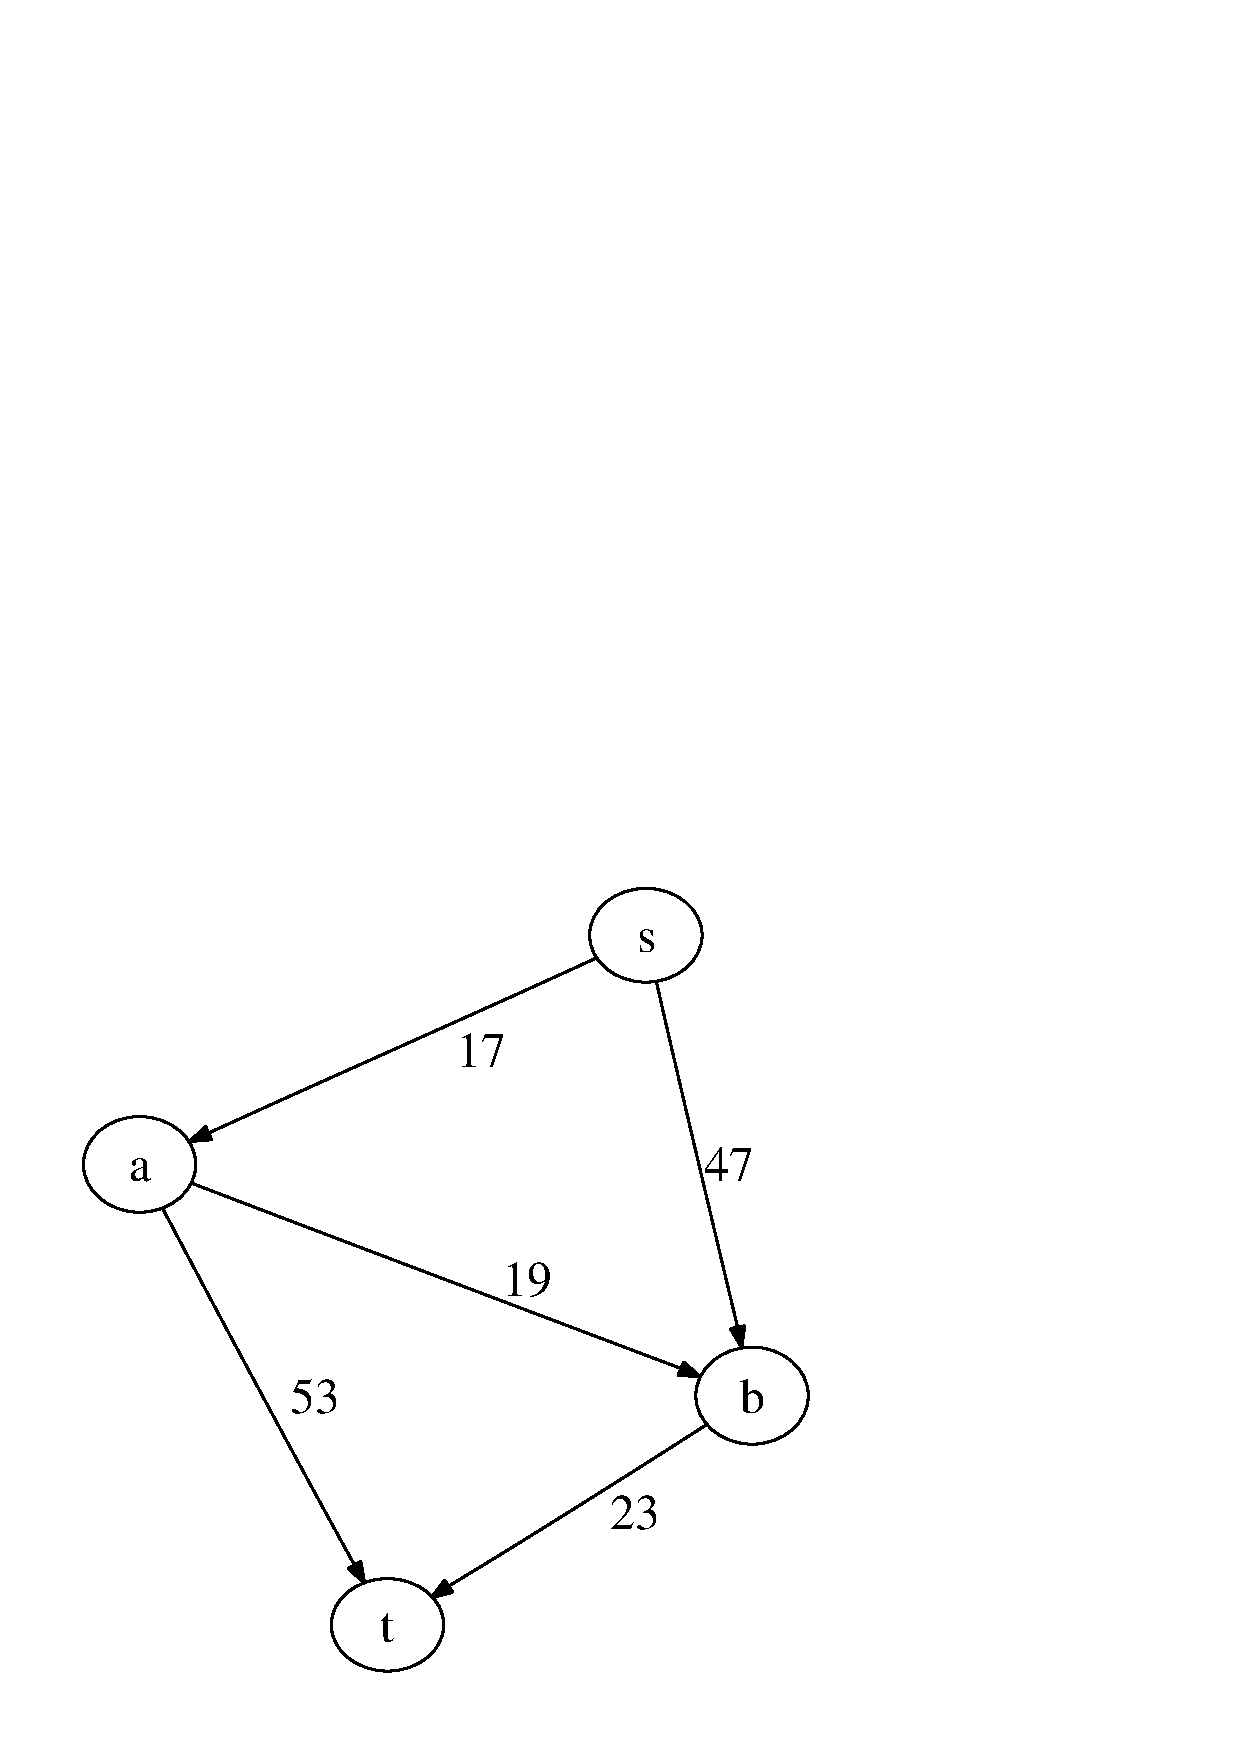
\includegraphics[height=4cm]{stexample}
  \end{center}
\end{minipage}
%
\begin{minipage}[c]{0.5\linewidth}
  $$
   \begin{array}{rll}
    \min& 17 x_{sa} + 47 x_{sb} + 19 x_{ab} + 53 x_{at} + 23 x_{bt}     \\
    \mbox{subject to}& x_{sa} = x_{ab} + x_{at} \\
    & x_{sb} + x_{ab} = x_{bt} \\
    &x_{ij} \in \{0,1\}, \mbox{for all {i,j}}\\
  \end{array}
  $$
\end{minipage}

The standard format used to feed such a problem into a solver is
called \mps which was invented by \ibm for the Mathematical
Programming System/360 in the
sixties~\cite{Kallrath2004b,Spielberg2004}.  Nearly all available \lp
and \mip solvers can read this format.  While \mps is a nice format to
punch into a punch card and at least a reasonable format to read for a
computer, it is quite unreadable for humans. For instance, the \mps
file of the above linear program looks as follows:


\lstset{language=mps,%
basicstyle=\sffamily\footnotesize,%
numberstyle=\sffamily\tiny\color{siennabrown},stepnumber=1}
\begin{lstlisting}[frame=]{}
NAME          shortestpath.lp                                                             
ROWS                                                                                   
 N  Obj                                                                                
 E  c0                                                                                 
 E  c1                                                                                 
 E  c2                                                                                 
COLUMNS                                                                                
    INTSTART  'MARKER'       'INTORG'          
    x0        Obj        17  c0            1   
    x0        c2          1                    
    x1        Obj        47  c1            1   
    x1        c2          1                    
    x2        c1          1  c0           -1   
    x2        Obj        19                    
    x3        Obj        53  c0           -1   
    x4        c1         -1  Obj          23   
RHS                                            
    RHS       c2          1                    
BOUNDS                                         
 UP Bound     x0          1                    
 UP Bound     x1          1                    
 UP Bound     x2          1                    
 UP Bound     x3          1                    
 UP Bound     x4          1                    
ENDATA                                                                                 
\end{lstlisting}

\bigskip
\noindent Another possibility is the \lpf format \cite{CPlex80} which
is more readable\footnote{ The \lpf format has also some idiosyncratic
  restrictions. For example variables should not be named \code{e12}
  or the like. and it is not possible to specify ranged
  constraints.}, quite similar to the instantiation, 
but only supported by a few solvers:
{ \small
\begin{verbatim}
Minimize
 Obj: +17 x0 +47 x1 +19 x2 +53 x3 +23 x4
Subject to
 c0: -1 x3 -1 x2 +1 x0 = +0
 c1: -1 x4 +1 x2 +1 x1 = +0
 c2: +1 x1 +1 x0 = +1
Bounds
 0 <= x0 <= 1
 0 <= x1 <= 1
 0 <= x2 <= 1
 0 <= x3 <= 1
 0 <= x4 <= 1
Generals
 x0 x1 x2 x3 x4
End
\end{verbatim}
}
\noindent Since each coefficient of the matrix~$A$ must be stated
explicitly it is also not a desirable choice for the development of a
mathematical model.

\subsubsection{Abstract formulation}

Now, with \zimpl it is possible to write 

{\small
\begin{verbatim}
set V      :={"a","b","s","t"};
set A      :={<"s","a">, <"s","b">, <"a","b">, <"a","t">, <"b","t">};
param c[A] := <"s","a"> 17, <"s","b"> 47, <"a","b"> 19, <"a","t"> 53,
              <"b","t"> 23;
defset dminus(v) := {<i,v> in A};
defset dplus(v)  := {<v,j> in A};
var x[A] binary;
minimize cost: sum<i,j> in A: c[i,j] * x[i,j];
subto fc:
      forall <v> in V - {"s","t"}:
        sum<i,v> in dminus(v): x[i,v] == sum<v,i> in dplus(v): x[v,i];
subto uf:
      sum<s,i> in dplus("s"): x[s,i] == 1;
\end{verbatim}
}

\noindent -- compare this with~(\ref{eq:shortestpath}). Feeding the
script into \zimpl will automatically generate \mps or \lpf files.


\medskip

The value of modeling languages like \zimpl lies in their ability to
work directly on the mathematical model in lieu of dealing merely with
coefficients. Furthermore, more often than not instantiations (read
\lpf or \mps-files) of models are generated from some external
data. In some sense, these are the result of the model applied to this
external data. In our example above, the external data is the graph
together with the cost coefficients and the specification of $s$ and
$t$, and the model is the formulation of the shortest $st$-path
problem. Of course, \zimpl supports the initialization of models
from files. For instance, the first lines from the \zimpl script above
can be replaced by {\small
\begin{verbatim}
set       V:= {read "nodes.txt" as "<1s>"};
set       A:= {read "arcs.txt"  as "<1s,2s>"};
param c[A] := read "arcs.txt"  as "<1s,2s>3n";
\end{verbatim}
} and the \zimpl script is ready produce instances of any shortest
path problem defined by the files ``nodes.txt'' and ``arcs.txt''. The
format of those files will be described in Subsection~\ref{initfromfile}.

\section{Invocation}

In order to run \zimpl on a model given in the file \code{ex1.zpl} type the command:
\begin{verbatim}
   zimpl ex1.zpl
\end{verbatim}
In general terms the command is:
\begin{verbatim}
   zimpl [options] <input-files>
\end{verbatim}
It is possible to give more than one input file. They are read one
after the other as if they were all one big file.
If any error occurs while processing, \zimpl prints out an 
error message and aborts. In case everything goes well, the results 
are written into two or more files, depending on the specified options.

The first output file is the problem generated from the model in either 
\cplex \lp, \mps, or  a ``human readable'' format, 
with extensions \emph{.lp}, \emph{.mps}, or \emph{.hum}, respectively.
The next one is the \emph{table} file which has the extension \emph{.tbl}.
The table file lists all variable and constraint names used in the model 
and their corresponding names in the problem file. 
The reason for this name translation is the limitation of the length
of names in the \mps format to 
eight characters. Also the \lp format
restricts the length of names. The precise limit is depending on the
version. \cplex~7.0 has a limit of 16 characters, and ignores
silently the rest of the name, while \cplex~9.0 has a limit of 255
characters, but will for some commands only show the first 20 characters 
in the output.

%The third file is and optional \cplex branching order file.

A complete list of all options understood by \zimpl can be found in
Table~\ref{tab:zimpl-options}. 
A typical invocation of \zimpl is for example:
\begin{verbatim}
   zimpl -o solveme -t mps data.zpl model.zpl
\end{verbatim}
This reads the files data.zpl and model.zpl as
input and produces as output the files solveme.mps and solveme.tbl.
Note that in case \mps-output is specified for a maximization problem,
the objective function will be inverted, because the \mps format has no
provision for stating the sense of the objective function. The default
is to assume minimization.

\begin{table}[hbtp]
{\sffamily\small\centering
\begin{tabular}{lp{104mm}}
\toprule
-t \emph{format} & Selects the output format. Can be either \code{lp},
                  which is default, or \code{mps}, or \code{pip},
                  which is polynomial IP,
                  or \code{hum}, which
                  is only human readable, or \code{rlp}, which is the
		  same as \code{lp} but with rows and columns randomly
                  permuted. The permutation is depending on the
		  \emph{seed}. Also possible is \code{pip}m which
		  means Polynomial IP.\\
-o \emph{name}   & Sets the base-name for the output files.\\ 
                & Defaults to the name of the first input file with 
                  its path and extension stripped off.\\ 
-F \emph{filter} & The output is piped through a filter. A \%s in the
                  string is replaced by the output filename. For example 
                  \code{-F "gzip -c >\%s.gz"} would compress all the 
                  output files.\\
-l \emph{length} & Sets maximal length of variables and
                  constraints for \code{lp} format files to \emph{length}.\\
-n \emph{cform}  & Select the format for the generation of constraint
                  names. Can be \code{cm} which will number them 
                  $1\ldots n$ with a `c' in front. \code{cn} will use 
                  the name supplied in the \code{subto} statement and 
                  number them $1\ldots n$ within the statement. 
                  \code{cf} will use the name given with the \code{subto},
                  then a $1\ldots n$ number like in \code{cm} and then 
                  append all the local variables from the forall statements.\\
-P \emph{filter} & The input is piped through a filter. A \%s in the
                  string is replaced by the input filename. For example 
                  \code{-P "cpp -DWITH\_C1 \%s"} would pass the input
		  file through the C-preprocessor.\\
-s \emph{seed}   & Positive \code{seed} number for the random number generator.
                 For example, \code{-s `date +\%N`} will produce changing random numbers.\\
-v \emph{0..5}   & Set the verbosity level. 0 is quiet, 1 is default,
                  2 is verbose, 3 and 4 are chatter, and 5 is debug.\\
-D \emph{name=val} & Sets the parameter \emph{name} to the specified
                  value. This is equivalent to having this line in the
                  \zimpl program: \code{param name:=val}. If there is
		  a declaration in the \zimpl file and a \code{-D}
		  setting for the same name, the latter takes precedent.\\
%\hline
-b & Enables bison debug output.\\
-f & Enables flex debug output.\\
-h & Prints a help message.\\
-m & Writes a \cplex \code{mst} (Mip STart) file.\\
-O & Tries to reduce the generated LP by doing some presolve analysis.\\
-r & Writes a \cplex \code{ord} branching order file.\\
-V & Prints the version number.\\
\bottomrule
\end{tabular}
}
\caption{\zimpl options}
\label{tab:zimpl-options}
\end{table}

% -----------------------------------------------------------------------------
% --- Format
% -----------------------------------------------------------------------------
\section{Format}

Each \zpl-file consists of six types of statements: 
\begin{itemize}
\setlength{\itemsep}{0pt}%
\item Sets
\item Parameters
\item Variables
\item Objective
\item Constraints
\item Function definitions
\end{itemize}
%
Each statement ends with a semicolon. 
Everything from a hash-sign \code{\#}, provided it is not part of a string, to 
the end of the line is treated as a
comment and is ignored.
If a line starts with the word \code{include} followed by a filename in double
quotation marks, then this file is read and processed instead of the line.

%-----------------------------------------------------------------------------------------
\subsection{Expressions}
%-----------------------------------------------------------------------------------------
\zimpl works on its lowest level with two types of data: Strings and
numbers. 
Wherever a number or string is required it is also possible to use a
parameter of the corresponding value type. In most cases, expressions are
allowed instead of just a number or a string.
The precedence of operators is the usual one, but
parentheses can always be used to specify the evaluation order explicitly.
%If in doubt use parenthesis.

\subsubsection{Numeric expressions}
A number in \zimpl can be given in the usual format, \eg as 2, -6.5 or 5.234e-12. 
Numeric expressions consist of numbers, numerically valued parameters, and
any of the operators and functions listed in Table~\ref{tab:zimpl-functions}.
Additionally the functions shown in Table~\ref{tab:zimpl-double} can be
used. Note that those functions are only computed with normal double precision
floating-point arithmetic and therefore have limited
accuracy. Examples on how to use the \code{min} and \code{max}
functions can be found in Section~\ref{ssec:parameters} on page~\pageref{ssec:parameters}. 

\begin{table}[hbtp]
\centering
{\sffamily\small
\begin{tabular}{lll}
\toprule
\code{a${}^\wedge$b}, \code{a**b} &$a$ to the power of $b$   & $a^b$, $b$ must be integer\\
\code{a+b}                       &addition                  & $a+b$\\
\code{a-b}                       &subtraction               & $a-b$\\
\code{a*b}                       &multiplication            & $a\cdot b$\\
\code{a/b}                       &division                  & $a/b$\\
\code{a mod b}                   &modulo                    & $a\mod b$\\
%\code{a div b}                   &integer division           & \\
\code{abs(a)}                    &absolute value            & $|a|$\\
\code{sgn(a)}                    &sign                      &
$x>0\Rightarrow 1, x<0\Rightarrow -1,\text{else }0$\\
\code{floor(a)}                  &round down                & $\lfloor a\rfloor$\\
\code{ceil(a)}                   &round up                  & $\lceil a\rceil$\\
\code{round(a)}                  &round towards zero        & $\lfloor a \rceil$\\
\code{a!}                        &factorial                 & $a!$,
$a$ must be nonnegative integer \\
\code{min(S)}                    &minimum of a set          &$\min_{s\in S}$\\
\code{min(s in S) e(s)}         &minimum over a set        &$\min_{s\in S} e(s)$\\
\code{max(S)}                    &maximum of a set          &$\max_{s\in S}$\\
\code{max(s in S) e(s)}         &maximum over a set        &$\max_{s\in S} e(s)$\\
\code{min(a,b,c,\ldots,n)}       &minimum of a list         &$\min (a,b,c,\ldots,n)$\\
\code{max(a,b,c,\ldots,n)}       &maximum of a list         &$\max (a,b,c,\ldots,n)$\\
\code{sum(s in S) e(s)}         &sum over a set            &$\sum_{s\in S} e(s)$\\
\code{prod(s in S) e(s)}        &product over a set        &$\prod_{s\in S} e(s)$\\
\code{card(S)}                   &cardinality of a set      &$|S|$\\
\code{random(m,n)}               & pseudo random number     &$\in[m,n]$, rational \\
\code{ord(A,n,c)}                &ordinal                   &c-th component of the n-th\\ 
                                 &                          & element of set $A$.\\
\code{length(s)}                 &length of a string        &number of characters in $s$\\
\code{if a then b}               &                          &\\
\code{else c end}        &\raisebox{1ex}[0cm][0cm]{conditional}
   &\raisebox{1ex}[0cm][0cm]{$\left\{\begin{array}{rl}b,&\text{if }
   a=\text{true}\\c,&\text{if } a=\text{false}\end{array}\right.$}\\\\
\bottomrule
\end{tabular}
}
\caption{Rational arithmetic functions}
\label{tab:zimpl-functions}
\end{table}

%With $\min$ and $\max$ it is possible to find the minimum/maximum
%member of an one dimensional set of numeric values.
%\code{card} gives the cardinality of a set.

\begin{table}[hbtp]
\centering
{\sffamily\small
\begin{tabular}{lll}
\toprule
\code{sqrt(a)}                   &square root               & $\sqrt a$\\
\code{log(a)}                    &logarithm to base 10      & $\log_{10}a$\\
\code{ln(a)}                     &natural logarithm         & $\ln a$\\
\code{exp(a)}                    &exponential function      & $e^a$\\
%\code{random(a,b)}               &random number in $\left[a,b\right]$&\\
\bottomrule
\end{tabular}
}
\caption{Double precision functions}
\label{tab:zimpl-double}
\end{table}

\subsubsection{String expressions}
A string is delimited by double quotation marks \code{"},
\eg\ \code{"Hallo Keiken"}. Two strings can be concatenated using the
\code{+} operator, \ie\ \code{"Hallo " + "Keiken"} gives \code{"Hallo
  Keiken"}. The function \code{substr(string, begin, length)} 
can be used to extract parts of a string. \code{begin} is the first character 
to be used, and counting starts with zero at first character. 
If \code{begin} is negative, then counting starts
at the end of the string. \code{length} is the number of charaters to extract 
starting at \code{begin}. The length of a string can be determined
using the \code{length} function.


\subsubsection{Boolean expressions}
These evaluate either to \emph{true} or to \emph{false}. For numbers and
strings the
relational operators $<$, $<=$, $==$, $!\!\!=$, $>=$, and $>$ are
defined.
Combinations of Boolean expressions with \code{and},
\code{or}, and 
\code{xor}\footnote{$a \text{ xor } b :=a\wedge\neg b\vee \neg a\wedge b$} 
and negation with \code{not} are possible.
The expression \emph{tuple} \code{in} \emph{set-expression} (explained
in the next section) can be used to test set membership of a tuple. 
Boolean expressions can also be in the \emph{then} or \emph{else} part of an 
\emph{if} expression.

\subsubsection{Variant expressions}
The following is either a numeric, string or boolean expression, depending on
whether \emph{expression} is a string, boolean, or numeric expression:

\smallskip
\code{if} \emph{boolean-expression} \code{then}
\emph{expression} \code{else} \emph{expression} \code{end}

\smallskip
\noindent The same is true for the \code{ord(}{}\emph{set,
  tuple-number, component-number}\code{)} function which evaluates to
a specific element of a set (details about sets are covered below).


\subsection{Tuples and sets}

A tuple is an ordered vector of fixed dimension where each component
is either a number or a string. Sets consist of (a finite number of)
tuples. Each tuple is unique within a set. All sets in \zimpl are
internally ordered, but there is no particular order.  Sets are
delimited by braces, \code{\{} and~\code{\}}, respectively.  All
tuples of a specific set have the same number of components.  The type
of the $n$-th component for all tuples of a set must be the same, \ie
they have to be either all numbers or all strings.  The definition of
a tuple is enclosed in angle brackets $<$ and $>$,
\eg\ \code{$<$1,2,"x"$>$}. The components are separated by commas.  If
tuples are one-dimensional, it is possible to omit the tuple
delimiters in a list of elements, but in this case they must be
omitted from all tuples in the definition, \eg\ \code{\{1,2,3\}} is
valid while \code{\{1,2,$<$3$>$\}} is not.

Sets can be defined with the set statement. It consists of
the keyword \code{set}, the name of the set, an assignment operator
\code{:=}, and a valid set expression.

Sets are referenced by the use of a \emph{template} tuple, consisting
of placeholders which are replaced by the values of the components of
the respective tuple. For example, a set $S$ consisting of two-dimensional
tuples could be referenced by \code{<a,b> in S}. If any of the
placeholders are actual values, only those tuples matching these
values will be extracted.
For example, \code{<1,b> in S} will only get
those tuples whose first component is \code{1}. Please note that if
one of the placeholders is the name of an already defined parameter,
set or variable, it will be substituted. This will result either in an
error or an actual value.

\paragraph{Examples}
{\small 
\begin{verbatim}
set A := { 1, 2, 3 };
set B := { "hi", "ha", "ho" };
set C := { <1,2,"x">, <6,5,"y">, <787,12.6,"oh"> };
\end{verbatim}
}
\noindent For set expressions the functions and
operators given in Table~\ref{tab:zimpl-set-functions} are defined.

An example for the use of the \code{if} \emph{boolean-expression} \code{then}
\emph{set-expression} \code{else} \emph{set-expression} \code{end} can
be found on page~\pageref{sec:indexed-sets} together with the examples for indexed sets.

\paragraph{Examples}
{\small 
\begin{verbatim}
set D := A cross B;
set E := { 6 to 9 } union A without { 2, 3 }; 
set F := { 1 to 9 } * { 10 to 19 } * { "A", "B" };
set G := proj(F, <3,1>); 
# will give: { <"A",1>, <"A",2"> ... <"B",9> }
\end{verbatim}
}

\begin{table}[htbp]
\centering
{\sffamily\small
\begin{tabular}{llp{61mm}}
\toprule
\code{A*B},&\\
\code{A cross B}   &\raisebox{1ex}[0cm][0cm]{cross product} 
                   &\raisebox{1ex}[0cm][0cm]{$\{(x,y)\mid x\in A\wedge y\in B\}$}\medskip\\
\code{A+B},&\\
\code{A union B}   &\raisebox{1ex}[0cm][0cm]{union} 
                   &\raisebox{1ex}[0cm][0cm]{$\{x\mid x\in A\vee x\in B\}$}\medskip\\
\code{union <i>}&\\
\code{ in I: S}&\raisebox{1ex}[0cm][0cm]{ditto, of indexed sets} 
               &\raisebox{1ex}[0cm][0cm]{$\bigcup_{i\in I}S_i$} \medskip\\
\code{A inter B}   &intersection & $\{x\mid x\in A\wedge x\in B\}$\medskip\\
\code{inter <i>}&\\
\code{ in I: S}&\raisebox{1ex}[0cm][0cm]{ditto, of indexed sets} 
               &\raisebox{1ex}[0cm][0cm]{$\bigcap_{i\in I}S_i$} \medskip\\
\code{A$\setminus$B, A-B},&\\
\code{A without B} &\raisebox{1ex}[0cm][0cm]{difference} 
                   &\raisebox{1ex}[0cm][0cm]{$\{x\mid x\in A\wedge x\not\in B\}$}\medskip\\
\code{A symdiff B} &symmetric difference& 
   $\{x\mid (x\in A\wedge x\not\in B)\vee(x\in B\wedge x\not\in A)\}$\\
\code{\{n\,{..}\,m \emph{by s}\}},& generate, &
   $\{x\mid x=\min(n,m) + i|s| \leq \max(n,m),$\\
   &(default $s = 1$) & $i\in\NN_0, x,n,m,s\in\ZZ\}$\\
\code{\{n to m \emph{by s}\}}&generate & 
   $\{x\mid x=n + is \leq m, i\in\NN_0, x,n,m,s\in\ZZ\}$\\
\code{proj(A, t)}& projection & 
   The new set will consist of $n$-tuples, with\\
   &$t=(e_1,\ldots,e_n)$&
   the $i$-th component being the $e_i$-th component of $A$.\\
\code{argmin <i>}&\\
\code{ in I : e(i)} & \raisebox{1ex}[0cm][0cm]{minimum argument} 
   &$\argmin_{i\in I} e(i)$\medskip\\
\code{argmin(n) <i>} & $n$ minimum
   & The new set consists\\
\code{ in I : e(i)} &  arguments 
   &of those $n$ elemens of $i$ for which $e(i)$ was
     smallest. The result can be ambiguous.\\
\code{argmax <i>}&\\
\code{ in I : e(i)} & \raisebox{1ex}[0cm][0cm]{maximum argument} 
   &$\argmax_{i\in I} e(i)$\medskip\\
\code{argmax(n) <i>} & $n$ maximum 
   & The new set consists\\ 
\code{ in I : e(i)} & arguments 
   & of those $n$ elemens of $i$ for which $e(i)$ was
     biggest. The result can be ambiguous.\\
\code{if a then b}\\
\code{else c end}        &\raisebox{1ex}[0cm][0cm]{conditional}
   &\raisebox{1ex}[0cm][0cm]{$\left\{\begin{array}{rl}b,&\text{if }
   a=\text{true}\\c,&\text{if } a=\text{false}\end{array}\right.$}\\\\
\bottomrule
\end{tabular}
}
\caption{Set related functions}
\label{tab:zimpl-set-functions}
\end{table}

\subsubsection{Conditional sets}
It is possible to restrict a set to tuples that 
satisfy a Boolean expression. The expression given by the \code{with}
clause is evaluated for each tuple in the set and only tuples for
which the expression evaluates to \emph{true} are included in the new set.

\paragraph{Examples}
{\small 
\begin{verbatim}
set F := { <i,j> in Q with i > j and i < 5 };
set A := { "a", "b", "c" };
set B := { 1, 2, 3 };
set V := { <a,2> in A*B with a == "a" or a == "b" };
# will give: { <"a",2>, <"b",2> }
set W := argmin(3) <i,j> in B*B : i+j;
# will give: { <1,1>, <1,2>, <2,1> } 
\end{verbatim}
}

\subsubsection{Indexed sets}
\label{sec:indexed-sets}
It is possible to index one set with another set resulting in a set of sets.
Indexed sets are accessed by adding the index of the set in brackets
\code{[} and \code{]}, like \code{S[7]}. 
Table~\ref{tab:zimpl-idxset-fun} lists the available functions.
There are three possibilities how to assign to an indexed set:
\begin{itemize}
\setlength{\itemsep}{0pt}%
\item The assignment expression is a list of comma-separated pairs, 
      consisting of a tuple from the index set and a set expression to assign.
\item If an index tuple is given as part of the index, 
      \eg \verb|<i> in I|, the assignment is evaluated for each value
      of the index tuple.
\item By use of a function that returns an indexed set.
\end{itemize}

\subsubsection{Examples}
{\small 
\begin{verbatim}
set I           := { 1..3 };
set A[I]        := <1> {"a","b"}, <2> {"c","e"}, <3> {"f"};
set B[<i> in I] := { 3 * i };
set P[]         := powerset(I);
set J           := indexset(P);
set S[]         := subsets(I, 2);
set T[]         := subsets(I, 1, 2);
set K[<i> in I] := if i mod 2 == 0 then { i } else { -i } end;
set U           := union <i> in I : A[i];
set IN          := inter <j> in J : P[j]; # empty! 
\end{verbatim}
}

\begin{table}[htbp]
\centering
{\sffamily\small
\begin{tabular}{llp{5cm}}
\toprule
\code{powerset(A)}& generates all subsets of $A$&$\{X\mid X\subseteq A\}$\\
\code{subsets(A,n)}& generates all subsets of $A$\\
                    & with $n$ elements&$\{X\mid X\subseteq A\wedge |X|=n\}$\\
\code{subsets(A,n,m)}& generates all subsets of $A$\\
                    & with between $n$ and $m$ elements
                    &$\{X\mid X\subseteq A\wedge n\leq |X|\leq m\}$\\
\code{indexset(A)}&the index set of $A$&$\{1\ldots |A|\}$\\
\bottomrule
\end{tabular}
}
\caption{Indexed set functions}
\label{tab:zimpl-idxset-fun}
\end{table}

%------------------------------------------------------------------------------
\subsection{Parameters}
\label{ssec:parameters}
%------------------------------------------------------------------------------

Parameters are the way to define constants within \zimpl. They can be
declared with or without an index set. Without index a parameter is
just a single value which is either a number or a string. For indexed
parameters there is one value for each member of the set. It is
possible to declare a \emph{default} value.

Parameters are declared in the following way: 
The keyword \code{param} is followed by the name of the parameter
optionally followed by the index set in square brackets. 
Then, after the assignment operator, there is a list of pairs. The first element of each
pair is a tuple from the index set, while the second element is the value of
the parameter for this index.

\subsubsection{Examples}
{\small 
\begin{verbatim}
set A := { 12 .. 30 };
set C := { <1,2,"x">, <6,5,"y">, <3,7,"z"> };
param q := 5;
param u[A] := <13> 17, <17> 29, <23> 14 default 99;
param amin := min A;               # = 12
param umin := min <a> in A : u[a]; # = 14 
param mmax := max <i> in { 1 .. 10 } : i mod 5;
param w[C] := <1,2,"x"> 1/2, <6,5,"y"> 2/3;
param x[<i> in { 1 .. 8 } with i mod 2 == 0] := 3 * i;
\end{verbatim}
}
\noindent
Assignments do not need to be complete.  In the example, no value is
given for index \code{$<$3,7,"z"$>$} of parameter \code{w}. This is
correct as long as it is never referenced.

\subsubsection{Parameter tables}
It is possible to initialize multi-dimensional indexed parameters from
tables. This is especially useful for two-dimensional parameters.
The data is put in a table structure with \code{$|$} signs on each
margin. Then a headline with column indices has to be added, and one index
for each row of the table is needed. The column index has to be
one-dimensional, but the row index can be
multi-dimensional. The complete index for the entry is built by
appending the column index to the row index.
The entries are separated by commas. Any valid expression is
allowed here. As can be seen in the third example below, it is
possible to add a list of entries after the table.



\subsubsection{Examples}
{\small 
\begin{verbatim}
set I := { 1 .. 10 };
set J := { "a", "b", "c", "x", "y", "z" };

param h[I*J] :=   | "a", "c", "x", "z"   |
                |1|  12,  17, 99,     23 |
                |3|   4,   3,-17, 66*5.5 |
                |5| 2/3, -.4,  3, abs(-4)|
                |9|   1,   2,  0,      3 | default -99;

param g[I*I*I] :=     | 1, 2, 3 |
                  |1,3| 0, 0, 1 | 
                  |2,1| 1, 0, 1 |;

param k[I*I] :=  |  7,  8,  9 |
               |4| 89, 67, 55 |
               |5| 12, 13, 14 |, <1,2> 17, <3,4> 99;
\end{verbatim}
}
\noindent The last example is equivalent to:
{\small 
\begin{verbatim}
param k[I*I] := <4,7> 89, <4,8> 67, <4,9> 55, <5,7> 12, 
                <5,8> 13, <5,9> 14, <1,2> 17, <3,4> 99;
\end{verbatim}
}

%------------------------------------------------------------------------------
\subsection{Initializing sets and parameters from a file}\label{initfromfile}
%------------------------------------------------------------------------------
It is possible to load the values for a set or a parameter from a
file. The syntax is:

\smallskip
\code{read} \emph{filename} \code{as} \emph{template} 
[\code{skip} \emph{n}] [\code{use} \emph{n}] 
[\code{match} \emph{s}] [\code{comment} \emph{s}]

\smallskip
\noindent\emph{filename} is the name of the file to read.
\emph{template} is a string with a template for the tuples to
generate. Each input line from the file is split into fields. The
splitting is done according to the following rules:
All leading and trailing space and tab characters in the line are removed.
Whenever a space, tab, comma, semicolon or colon is encountered
a new field is started. Text that is enclosed in double quotes is not
split and the quotes are always removed. When a field is split all space
and tab characters around the splitting point are removed. 
If the split is
due to a comma, semicolon or colon, each occurrence of these
characters starts a new field. 

\subsubsection{Examples}
All these lines have three fields:
{\small 
\begin{verbatim}
Hallo;12;3    
Moin   7  2
"Hallo, Peter"; "Nice to meet you" 77
,,2
\end{verbatim}
}

\noindent For each component of the tuple, the number of the field
to use for the value is given, followed by either \code{n} if the
field should be interpreted as a number or \code{s} for a string. 
After the template, some optional modifiers can be given. The order
does not matter. 
\code{match} \emph{s} compares the regular expression \emph{s} against
the line read from the file. Only if the expression matches the 
line, it is processed further. POSIX extended regular expression syntax
is used.
\code{comment} \emph{s} sets a list of characters that start
comments in the file. Each line is ended when any of the comment
characters is found.
\code{skip} \emph{n} instructs to skip the first
\emph{n} lines of the file. 
\code{use} \emph{n} limits the number of
lines to use to \emph{n}. 
When a file is read, empty lines, comment lines, and unmatched lines
are skipped and not counted for the \code{use} and \code{skip} clauses.
 
\subsubsection{Examples}
{\small
\verb|set P := { read "nodes.txt" as "<1s>" };|

\smallskip
\noindent\verb|nodes.txt:|\\
\verb|   Hamburg            | $\rightarrow$ $<$"Hamburg"$>$\\
\verb|   M�nchen            | $\rightarrow$ $<$"M�nchen"$>$\\
\verb|   Berlin             | $\rightarrow$ $<$"Berlin"$>$\\

\smallskip
\noindent\verb|set Q := { read "blabla.txt" as "<1s,5n,2n>" skip 1 use 2 };|

\smallskip
\noindent\verb|blabla.txt:|\\
\verb|   Name;Nr;X;Y;No     | $\rightarrow$ skip\\   
\verb|   Hamburg;12;x;y;7   | $\rightarrow$ $<$"Hamburg",7,12$>$\\
\verb|   Bremen;4;x;y;5     | $\rightarrow$ $<$"Bremen",5,4$>$\\
\verb|   Berlin;2;x;y;8     | $\rightarrow$ skip\\
   
\smallskip
\noindent\verb|param cost[P] := read "cost.txt" as "<1s> 2n" comment "#";|

\smallskip
\noindent\verb|cost.txt:|\\
\verb|   # Name Price       | $\rightarrow$ skip\\
\verb|   Hamburg 1000       | $\rightarrow$ $<$"Hamburg"$>$ 1000\\
\verb|   M�nchen 1200       | $\rightarrow$ $<$"M�nchen"$>$ 1200\\
\verb|   Berlin  1400       | $\rightarrow$ $<$"Berlin"$>$ 1400\\

\smallskip
\noindent\verb|param cost[Q] := read "haha.txt" as "<3s,1n,2n> 4s";|

\smallskip
\noindent\verb|haha.txt:|\\
\verb|      1:2:ab:con1     | $\rightarrow$ $<$"ab",1,2$>$ "con1"\\
\verb|      2:3:bc:con2     | $\rightarrow$ $<$"bc",2,3$>$ "con2"\\
\verb|      4:5:de:con3     | $\rightarrow$ $<$"de",4,5$>$ "con3"\\
}  

\noindent As with table format input, it is possible to add a list of tuples or
parameter entries after a read statement.
\subsubsection{Examples}
{\small 
\begin{verbatim}
set A := { read "test.txt" as "<2n>", <5>, <6> }; 
param winniepoh[X] := 
   read "values.txt" as "<1n,2n> 3n", <1,2> 17, <3,4> 29;
\end{verbatim}
}  

It is also possible to read a single value into a parameter. In this
case, either the file should contain only a single line, or the read
statement should be instructed by means of a \code{use 1} parameter
only to read a single line.

\subsubsection{Examples}
{\small 
\begin{verbatim}
# Read the fourth value in the fifth line
param n := read "huhu.dat" as "4n" skip 4 use 1;
\end{verbatim}
}  

If all values in a file should be read into a set, this is possible by
use of the \code{"<s+>"} template for string values, and \code{"<n+>"}
for numerical values. Note, that currently at most 65536 values are allowed in a
single line. 


\subsubsection{Examples}
{\small 
\begin{verbatim}
# Read all values into a set
set X := { read "stream.txt" as "<n+>" };

stream.txt:
1 2 3 7 9 5 6 23 
63 37 88 
4
87 27  

# X := { 1, 2, 3, 7, 9, 5, 6, 23, 63, 37, 88, 4, 87, 27 };
\end{verbatim}
}  

\subsection{\emph{sum}-expressions }
%------------------------------------------------------------------------------
Sums are stated in the form:

\smallskip
\code{sum} \emph{index} \code{do} \emph{term}

\smallskip 
\noindent It is possible to nest several sum instructions, but it is
probably more convenient to simply merge the indices.
The general form of \emph{index} is: 

\smallskip
\emph{tuple} \code{in} \emph{set} \code{with} \emph{boolean-expression}

\smallskip
\noindent It is allowed to write a colon \code{:} instead of \code{do} and a
vertical bar \code{|} instead of \code{with}.
The number of components in the \emph{tuple} and in the
members of the \emph{set} must match. The \code{with} part of an \emph{index} is
optional. The \emph{set} can be any expression giving a set. Examples
are given in the next section.

%------------------------------------------------------------------------------
\subsection{\emph{forall}-statements}
%------------------------------------------------------------------------------
The general forms are:

\smallskip
\code{forall} \emph{index} \code{do} \emph{term}

\smallskip 
\noindent It is possible to nest several forall instructions.
%It should be noted, that a \code{sum}-expression is a \emph{term}
%itself, so it is possible to nest or concatenate them.
The general form of \emph{index} equals that of
\emph{sum}-expressions.  Examples are given in the next section.

%------------------------------------------------------------------------------
\subsection{Function definitions}
%------------------------------------------------------------------------------
It is possible to define functions within \zimpl. The value a
function returns has to be either a number, a string, a boolean, or a set.
The arguments of a function can only be numbers or strings, but within
the function definition it is possible to access all otherwise
declared sets and parameters.

The definition of a function has to start with 
\code{defnumb}, \code{defstrg}, \code{defbool}, or \code{defset}, depending on the
return value.
Next is the name
of the function and a list of argument names put in parentheses.
An assignment operator \code{:=} has to follow and a valid
expression or set expression.

\subsubsection{Examples}
{\small 
\begin{verbatim}
defnumb dist(a,b)     := sqrt(a*a + b*b);
defstrg huehott(a)    := if a < 0 then "hue" else "hott" end;
defbool wirklich(a,b) := a < b and a >= 10 or b < 5; 
defset  bigger(i)     := { <j> in K with j > i };
\end{verbatim}
}


%------------------------------------------------------------------------------
\subsection{The \emph{do print} and \emph{do check} commands}
%------------------------------------------------------------------------------
The \code{do} command is special.
It has two possible incarnations:
\code{print} and \code{check}. \code{print} will print to the 
standard output stream
whatever numerical, string, Boolean or set expression, or tuple
follows it. This can be used for example to check if a set has the
expected members, or if some computation has the anticipated result.
\code{check} always precedes a Boolean expression. If this
expression does not evaluate to \emph{true}, the program is aborted
with an appropriate error message. This can be used to assert that
specific conditions are met.
It is possible to use a \code{forall} clause before a \code{print}
or \code{check} statement.
For string and numeric values, it is possible to give a comma-separated
list to the print statement.

\subsubsection{Examples}
{\small 
\begin{verbatim}
set I := { 1..10 };
do print I;
do print "Cardinality of I:", card(I);
do forall <i> in I with i > 5 do print sqrt(i);
do forall <p> in P do check sum <p,i> in PI : 1 >= 1;
\end{verbatim}
}



%------------------------------------------------------------------------------
\section{Models}
%------------------------------------------------------------------------------
In this section, we use the machinery developed up to now to
formulate mathematical programs. Apart from the usual syntax to
declare variables, objective functions and constraints there is
special syntax available that permits the easy formulation of special
constraints, such as special ordered sets, conditional constraints,
and extended functions.

\subsection{Variables}
%------------------------------------------------------------------------------
Like parameters, variables can be indexed. 
A variable has to be one out of three possible types: 
Continuous (called \code{real}), \code{binary} or \code{integer}. The default type is real. 
Variables may have lower and upper bounds. Defaults are
zero as the lower and infinity as the upper bound. Binary variables are
always bounded between zero and one.
It is possible to compute the value of the lower or upper bounds
depending on the index of the variable (see the last declaration in the
example). Bounds can also be set to \code{infinity} and \code{-infinity}.
Binary and integer variables can be declared \code{implicit}, \ie the
variable can be assumed to have an integral value in any optimal
solution to the integer program, even if it is declared continuous. 
Use of \emph{implicit} is only useful if used together with a solver
that take advantage of this information. As of this writing, only \scip
(\url{http://scip.zib.de}) with linked in \zimpl can do so.
In all other cases, the variable is treated as a continuous variable. 
It is possible to specify initial values for integer variables by use
of the \code{startval} keyword. Furthermore, the branching  priority
can be given using the \code{priority} keyword. Currently, these
values are written to a \cplex \code{ord} branching order file if the
\code{-r} command line switch is given.

\subsubsection{Examples}
{\small 
\begin{verbatim}
var x1;
var x2 binary;
var x3 integer >= -infinity      # free variable
var y[A] real >= 2 <= 18;
var z[<a,b> in C] integer 
      >= a * 10 <= if b <= 3 then p[b] else infinity end; 
var w implicit binary;
var t[k in K] integer >= 1 <= 3 * k startval 2 * k priority 50;
\end{verbatim}
}

%\fbox{Remember: if nothing is specified a lower bound of zero is assumed.}


\subsection{Objective}
There must be at most one objective statement in a model. The objective
can be either \code{minimize} or \code{maximize}. Following the
keyword is a name, a colon : and then a linear term expressing the
objective function.

If there is an objective offset, \ie a constant value in the
objective function, \zimpl automatically generates an internal
variable \code{@@ObjOffset} set to one. This variable is put into the
objective function with the appropriate coefficient.\footnote{The reason for
this is that there is no portable way to put an offset into the
objective function in neither \lpf nor \mps-format.}

\subsubsection{Example}
{\small 
\begin{verbatim}
minimize cost: 12 * x1 -4.4 * x2 + 5
   + sum <a> in A : u[a] * y[a]
   + sum <a,b,c> in C with a in E and b > 3 : -a/2 * z[a,b,c];
maximize profit: sum <i> in I : c[i] * x[i];
\end{verbatim}
}

%------------------------------------------------------------------------------
\subsection{Constraints}\label{ssec:ug:constraints}
%------------------------------------------------------------------------------
The general format for a constraint is:

\smallskip
\verb|subto name: term sense term|

\smallskip
\noindent Alternatively, it is also possible to define \emph{ranged} constraints 
which have the form:

\smallskip
\verb|subto name: expr sense term sense expr|

\smallskip
\noindent \code{name} can be any name starting with a letter. \code{term} is defined
as in the objective. \code{sense} is one of
\code{<=}, \code{>=} and \code{==}. In case of ranged constraints
both senses have to be equal and may not be \code{==}. \code{expr} is any
valid expression that evaluates to a number.

Additional to linear constraints as in the objective it is also
possible to state terms with higher degree for constraints.

Many constraints can be generated with one statement by the use of the
\code{forall} instruction, as shown below.

\subsubsection{Examples}
{\small 
\begin{verbatim}
subto time:  3 * x1 + 4 * x2 <= 7;
subto space: 50 >= sum <a> in A: 2 * u[a] * y[a] >= 5;
subto weird: forall <a> in A: sum <a,b,c> in C: z[a,b,c]==55;
subto c21: 6*(sum <i> in A: x[i] + sum <j> in B : y[j]) >= 2;
subto c40: x[1] == a[1] + 2 * sum <i> in A do 2*a[i]*x[i]*3+4;
subto frown: forall <i,j> in X cross { 1 to 5 } without { <2,3> }       
               with i > 5 and j < 2 do                                 
                  sum <i,j,k> in X cross { 1 to 3 } cross Z do         
                     p[i] * q[j] * w[j,k] >= if i == 2 then 17 else 53 end;
subto nonlin: 3 * x * y * z + 6 <= x^3 + z * y^2 + 3;
\end{verbatim}
}
\noindent Note that in the example \emph{i} and \emph{j} are set by the \code{forall}
instruction. So they are fixed in all invocations of \code{sum}.

%------------------------------------------------------------------------------
\subsubsection{\emph{if} in terms}
%------------------------------------------------------------------------------
Part of a constraint can be put into an \code{if-then-else-end}.
In this particular case, the else part is mandatory and both parts
need to include some variables in the term. 

\subsubsection{Examples}
{\small 
\begin{verbatim}
subto c2: sum <i> in I :
     if (i mod 2 == 0) then 3 * x[i] else -2 * y[i] end <= 3;
\end{verbatim}
}

%------------------------------------------------------------------------------
\subsubsection{\emph{if} in constraints}
%------------------------------------------------------------------------------
It is possible to put two variants of a constraint into an
\code{if}-statement. 
A \code{forall} statement inside the result part of an \code{if} is
also possible. The \code{else} part is optional.

\subsubsection{Examples}
{\small 
\begin{verbatim}
subto c1: forall <i> in I do
  if (i mod 2 == 0) then  3 * x[i] >= 4
                    else -2 * y[i] <= 3 end;
\end{verbatim}
}

%------------------------------------------------------------------------------
\subsubsection{Combining constraints with \emph{and}}
%------------------------------------------------------------------------------
It is possible to group constraints by concatenating them with
\code{and}. This group will then always be processed together.
This operator is particularly useful in combination with \code{forall} and \code{if}.

\subsubsection{Examples}
{\small 
\begin{verbatim}
subto c1: forall <i> in I:
  if (i > 3)
     then if (i == 4) 
        then z[1] + z[2] == i
        else z[2] + z[3] == i
     end and
     z[3] + z[4] == i and
     z[4] + z[5] == i
  else
     if (i == 2) 
        then z[1] + z[2] == i + 10
        else z[2] + z[3] == i + 10
     end and
     z[3] + z[4] == i + 10 and
     z[4] + z[5] == i + 10
  end;
\end{verbatim}
}


%------------------------------------------------------------------------------
\subsubsection{Constraint attributes}
%------------------------------------------------------------------------------
It is possible to specify special attributes for a constraint regarding
how it should be handled later on.

\begin{description}
\item[scale]
  Before the constraint is written to a file, it is scaled by 
  $1/\max |c|$ with $c$ being the coefficients of the constraint.
\item[separate]
  Do not include the constraint in the initial LP, but separate it later on.
  The constraint need not to be checked for feasibility.
  When written to an \lpf file it will be written into a \code{USER
  CUTS} section, in \scip separate will be set to true.
\item[checkonly]
  Do not include the constraint in the initial LP, but separate only to
  check for feasibility.
  When written to an \lpf file it will be written into a \code{LAZY
  CUTS} section, in \scip check will be set to true.
\item[indicator]
  If vif (see below) is part of the constraint then it is modeled as an 
  indicator constraint and not by a big-M formulation.
  If you use this attribute, you can no longer write \mps-format, as
  indicator variables are not supported by this format.
\end{description}

\noindent
The attributes are given after the constraint, before the semi-colon
and are separated by commas.

\subsubsection{Examples}
{\small 
\begin{verbatim}
subto c1: 1000 * x + 0.3 * y <= 5, scale, checkonly;
subto c2: x + y + z == 7, separate; 
subto c3: vif x == 1 then y == 7 end, indicator;
\end{verbatim}
}


%------------------------------------------------------------------------------
\subsubsection{Special ordered sets}
%------------------------------------------------------------------------------
\zimpl can be used to specify special ordered sets (\sos) for an
integer program. If a model contains any \sos a \code{sos} file is
written together with the \code{lp} or \code{mps} file.
The general format of a special ordered set is:

\smallskip
\verb@sos name: [type1|type2] priority expr : term@

\smallskip
\noindent \code{name} can be any name starting with a letter. \sos use
the same namespace as constraints.
\code{term} is defined as in the objective. \code{type1} or
\code{type2} indicate whether a type-1 or type-2 special ordered set
is declared. The priority is optional and equal to the priority
setting for variables.
Many \sos can be generated with one statement by the use of the
\code{forall} instruction, as shown above.

\subsubsection{Examples}
{\small 
\begin{verbatim}
sos s1: type1: 100 * x[1] + 200 * x[2] + 400 * x[3];
sos s2: type2 priority 100 : sum <i> in I: a[i] * x[i];
sos s3: forall <i> in I with i > 2: 
           type1: (100 + i) * x[i] + i * x[i-1];
\end{verbatim}
}

%------------------------------------------------------------------------------
\subsubsection{Extended constraints}
%------------------------------------------------------------------------------
\zimpl can generate systems of constraints that
mimic conditional constraints. The general syntax is as follows (note
that the \code{else} part is optional):

\smallskip
\centerline{
\code{vif} \emph{boolean-constraint} \code{then} \emph{constraint} 
[ \code{else} \emph{constraint} ] \code{end}}

\smallskip
\noindent where \emph{boolean-constraint} consists of a linear expression involving
variables. All these variables have to be bounded integer or binary
variables. It is not possible to use any continuous variables or integer
variables with infinite bounds in a \emph{boolean-constraint}.
All comparison operators ($<$, $\le$, $==$, $!\!\!=$, $\ge$, $>$) are
allowed. Also, the combination of several terms with \code{and},
\code{or}, and \code{xor} and negation with \code{not} is possible.
The conditional constraints (those which follow after \code{then} or
\code{else}) may include bounded continuous variables. 
Be aware that using this construct will lead to
the generation of several additional constraints and variables.

\subsubsection{Examples}
{\small 
\begin{verbatim}
var x[I] integer >= 0 <= 20;
subto c1: vif 3 * x[1] + x[2] != 7 
   then sum <i> in I : y[i] <= 17
   else sum <k> in K : z[k] >= 5 end;
subto c2: vif x[1] == 1 and x[2] > 5 then x[3] == 7 end;
subto c3: forall <i> in I with i < max(I) : 
   vif x[i] >= 2 then x[i + 1] <= 4 end;
\end{verbatim}
}

%------------------------------------------------------------------------------
\subsubsection{Extended functions}
%------------------------------------------------------------------------------
It is possible to use special functions on terms with variables that
will automatically be converted into a system of inequalities. The
arguments of these functions have to be linear terms consisting of
bounded integer or binary variables. At the moment only the function
\code{vabs(t)} that computes the absolute value of the term \code{t}
is implemented, but functions like the minimum or the maximum of two
terms, or the sign of a term can be implemented in a similar manner.
Again, using this construct will lead to
the generation of several additional constraints and variables.

\subsubsection{Examples}
{\small 
\begin{verbatim}
var x[I] integer >= -5 <= 5;
subto c1: vabs(sum <i> in I : x[i]) <= 15;
subto c2: vif vabs(x[1] + x[2]) > 2 then x[3] == 2 end;
\end{verbatim}
}




\clearpage
\section{Modeling examples}\label{modelingexamples}
In this section we show some examples of well-known problems
translated into \zimpl format.

\subsection{The diet problem}
This is the first example in 
\cite[Chapter 1, page 3]{Chvatal1983}.
It is a classic so-called \emph{diet} problem, see for example
\cite{Dantzig1990} about its implications in practice.

Given a set of foods $F$ and a set of nutrients $N$, we have a table
$\pi_{fn}$ of the amount of nutrient $n$ in food $f$. Now $\Pi_n$
defines how much intake of each nutrient is needed. $\Delta_f$
denotes for each food the maximum number of servings acceptable. 
Given prices $c_f$ for each food, we have to find a selection of foods
that obeys the restrictions and has minimal cost. An integer
variable $x_f$ is introduced for each $f\in F$ indicating the number of servings of
food $f$. Integer variables are used, because only complete servings can be
obtained, \ie half an egg is not an option.
The problem may be stated as:
\begin{align*}
\min&\sum_{f\in F}c_{f} x_{f}&&\mbox{subject to}\nonumber\\
\sum_{f\in F} \pi_{fn} x_{f}&\ge\Pi_n&&\fa n\in N\nonumber\\
0\leq x_{f}&\leq\Delta_f&&\fa f\in F\nonumber\\
x_{f}&\in\NNZ&&\fa f\in F
\end{align*}

\noindent This translates into \zimpl as follows:

\medskip
\lstset{language=zimpl,%
basicstyle=\sffamily\footnotesize,%
numberstyle=\sffamily\tiny\color{siennabrown},stepnumber=1}
\begin{lstlisting}[frame=tb]{}
set Food      := { "Oatmeal", "Chicken", "Eggs",
                   "Milk",    "Pie",     "Pork" };
set Nutrients := { "Energy",  "Protein", "Calcium" };
set Attr      := Nutrients + { "Servings", "Price" };

param needed[Nutrients] := 
   <"Energy"> 2000, <"Protein"> 55, <"Calcium"> 800;

param data[Food * Attr] := 
          |"Servings","Energy","Protein","Calcium","Price"|
|"Oatmeal"|        4 ,    110 ,       4 ,       2 ,     3 |
|"Chicken"|        3 ,    205 ,      32 ,      12 ,    24 |
|"Eggs"   |        2 ,    160 ,      13 ,      54 ,    13 |
|"Milk"   |        8 ,    160 ,       8 ,     284 ,     9 |
|"Pie"    |        2 ,    420 ,       4 ,      22 ,    20 |
|"Pork"   |        2 ,    260 ,      14 ,      80 ,    19 |;
#                       (kcal)       (g)      (mg) (cents)       

var x[<f> in Food] integer >= 0 <= data[f, "Servings"];

minimize cost: sum <f> in Food : data[f, "Price"] * x[f];

subto need: forall <n> in Nutrients do
   sum <f> in Food : data[f, n] * x[f] >= needed[n];
\end{lstlisting}

\medskip
\noindent The cheapest meal satisfying all requirements costs 97 cents and
consists of four servings of oatmeal, five servings of milk and two
servings of pie.

%x$Oatmeal                     4.000000
%x$Milk                        5.000000
%x$Pie                         2.000000

\subsection{The traveling salesman problem}
In this example, we show how to generate an exponential 
description of the \emph{symmetric traveling salesman problem} (\tsp)
as given for example in 
\cite[Section 58.5]{Schrijver2003}.

Let $G=(V,E)$ be a complete graph, with $V$ being the set of cities
and $E$ being the set of links between the cities. Introducing binary
variables $x_{ij}$ for each $(i,j)\in E$ indicating if edge $(i,j)$ is
part of the tour, the \tsp can be written as:
\begin{align*}
\min &\sum_{(i,j)\in E}d_{ij} x_{ij}&&\text{subject to}\nonumber\\
\sum_{(i,j)\in\delta_v} x_{ij}&=2&&\fa v\in V\nonumber\\
\sum_{(i,j)\in E(U)} x_{ij}&\leq |U|-1&&\fa U\subseteq V, \emptyset\neq
U\neq V\\
x_{ij}&\in\{0,1\}&&\fa (i,j)\in E\nonumber
\end{align*}
%
The data is read in from a file that gives the number of the city and the
x and y coordinates. Distances between cities are assumed Euclidean. For example:
{\footnotesize
\setlength\columnseprule{0.4pt}
\begin{multicols}{2}
\begin{verbatim}
# City       X    Y
Berlin     5251 1340
Frankfurt  5011  864 
Leipzig    5133 1237 
Heidelberg 4941  867 
Karlsruhe  4901  840 
Hamburg    5356  998 
Bayreuth   4993 1159 
Trier      4974  668 
Hannover   5237  972
Stuttgart  4874  909 
Passau     4856 1344 
Augsburg   4833 1089 
Koblenz    5033  759 
Dortmund   5148  741 
Bochum     5145  728 
Duisburg   5142  679 
Wuppertal  5124  715 
Essen      5145  701 
Jena       5093 1158 
\end{verbatim}
\end{multicols}
}

% {\small
% \begin{verbatim}
% #City        x y 
% "Sylt"       1 1
% "Flensburg"  3 1
% "Neum�nster" 2 2
% "Husum"      1 3
% "Schleswig"  3 3
% "Ausacker"   2 4
% \end{verbatim}
% }

\noindent The formulation in \zimpl follows below. Please note that \code{P[]}
holds all subsets of the cities. As a result 
19 cities is about as far as one can get with this approach. 
Information on how to solve much larger instances can be found on the 
\textsc{concorde} website\footnote{http://www.tsp.gatech.edu}.

\medskip
\lstset{language=zimpl,%
basicstyle=\sffamily\footnotesize,%
numberstyle=\sffamily\tiny\color{siennabrown},stepnumber=1}
\begin{lstlisting}[frame=tb]{}
set V             := { read "tsp.dat" as "<1s>" comment "#" };
set E             := { <i,j> in V * V with i < j };
set P[]           := powerset(V);
set K             := indexset(P);

param px[V]       := read "tsp.dat" as "<1s> 2n" comment "#";
param py[V]       := read "tsp.dat" as "<1s> 3n" comment "#";

defnumb dist(a,b) := sqrt((px[a]-px[b])^2 + (py[a]-py[b])^2);

var x[E] binary;

minimize cost: sum <i,j> in E : dist(i,j) * x[i, j];

subto two_connected: forall <v> in V do
   (sum <v,j> in E : x[v,j]) + (sum <i,v> in E : x[i,v]) == 2;

subto no_subtour: 
   forall <k> in K with 
      card(P[k]) > 2 and card(P[k]) < card(V) - 2 do
      sum <i,j> in E with <i> in P[k] and <j> in P[k] : x[i,j] 
      <= card(P[k]) - 1;
\end{lstlisting}

\medskip
\noindent The resulting \lp has 171 variables, 239,925 constraints, and
22,387,149 non-zero entries in the constraint matrix, giving an \mps-file
size of 936\,\textsc{mb}. \cplex solves this to optimality
without branching in less than a minute.\footnote{Only 40
simplex iterations are needed to reach the optimal solution.}

An optimal tour for the data above is 
Berlin, Hamburg, Hannover, Dortmund, Bo\-chum, Wuppertal, Essen,
Duisburg, Trier, Koblenz, Frankfurt, Heidelberg, Karlsruhe, Stuttgart,
Augsburg, Passau, Bayreuth, Jena, Leipzig, Berlin.


\subsection{The capacitated facility location problem}
Here we give a formulation of the \emph{capacitated facility
location} problem. It may also be considered as a kind of \emph{bin packing} problem
with packing costs and variable sized bins, or as a \emph{cutting stock} problem
with cutting costs.

Given a set of possible plants $P$ to build, and a set of stores $S$
with a certain demand $\delta_s$ that has to be satisfied, we have
to decide which plant should serve which store.
We have costs $c_p$ for building plant $p$ and $c_{ps}$
for transporting the goods from plant $p$ to store $s$.
Each plant has only a limited capacity $\kappa_p$.
We insist that each store is served by exactly one plant.
Of course we are looking for the cheapest solution:
%
\begin{align}
\min\sum_{p\in P}c_p z_p& 
   +\!\!\!\sum_{p\in P, s\in S}\!\!\!c_{ps} x_{ps}&&\mbox{subject to}\nonumber\\ 
\sum_{p\in P} x_{ps}& = 1&&\fa s\in S\label{eqn:assign}\\
x_{ps}&\leq z_{p}&&\fa s\in S, p\in P\label{eqn:open}\\
\sum_{s\in S} \delta_s x_{ps}&\leq\kappa_p&&\fa p\in P\label{eqn:capacity}\\
x_{ps},z_p&\in\BB&&\fa p\in P, s\in S\nonumber
\end{align}
%
We use binary variables $z_p$ which are set to one, if and only if plant $p$ is
to be built. Additionally, we have binary variables $x_{ps}$ 
which are set to one if and only if plant $p$ serves shop $s$. 
Equation~\eqref{eqn:assign} demands that each store is assigned to
exactly one plant. Inequality~\eqref{eqn:open} makes sure that a plant
that serves a shop is built. Inequality~\eqref{eqn:capacity}
assures that the shops are served by a plant which does not exceed its
capacity. Putting this into \zimpl yields the program shown on the
next page.
The optimal solution for the instance described by the program is to build plants \code{A} and
\code{C}. Stores 2, 3, and 4 are served by plant \code{A} and the others by
plant \code{C}. The total cost is 1457.

\clearpage
\lstset{language=zimpl,%
basicstyle=\sffamily\footnotesize,%
numberstyle=\sffamily\tiny\color{siennabrown},stepnumber=1}
\begin{lstlisting}[frame=]{}
set PLANTS := { "A", "B", "C", "D" };
set STORES := { 1 .. 9 };
set PS     := PLANTS * STORES;

# How much does it cost to build a plant and what capacity 
# will it then have?
param building[PLANTS]:= <"A"> 500, <"B"> 600, <"C"> 700, <"D"> 800;
param capacity[PLANTS]:= <"A">  40, <"B">  55, <"C">  73, <"D">  90;

# The demand for each store
param demand  [STORES]:= <1> 10, <2> 14,
                         <3> 17, <4>  8,
                         <5>  9, <6> 12,
                         <7> 11, <8> 15,
                         <9> 16;

# Transportation cost from each plant to each store
param transport[PS] := 
      |  1,  2,  3,  4,  5,  6,  7,  8,  9 |
  |"A"| 55,  4, 17, 33, 47, 98, 19, 10,  6 |
  |"B"| 42, 12,  4, 23, 16, 78, 47,  9, 82 | 
  |"C"| 17, 34, 65, 25,  7, 67, 45, 13, 54 |
  |"D"| 60,  8, 79, 24, 28, 19, 62, 18, 45 |;

var x[PS]     binary;  # Is plant p supplying store s ?
var z[PLANTS] binary;  # Is plant p built ?

# We want it cheap
minimize cost: sum <p> in PLANTS : building[p] * z[p]
             + sum <p,s> in PS : transport[p,s] * x[p,s];

# Each store is supplied by exactly one plant
subto assign: 
  forall <s> in STORES do 
     sum <p> in PLANTS : x[p,s] == 1;
   
# To be able to supply a store, a plant must be built
subto build: 
   forall <p,s> in PS do 
      x[p,s] <= z[p];

# The plant must be able to meet the demands from all stores
# that are assigned to it
subto limit: 
   forall <p> in PLANTS do
      sum <s> in S : demand[s] * x[p,s] <= capacity[p];
\end{lstlisting}
\clearpage

\subsection{The \emph{n}-queens problem}
\label{ssec:example:n-queens-problem}
The problem is to place $n$ queens on a $n\times n$ chessboard so that no
two queens are on the same row, column or diagonal.
The $n$-queens problem is a classic combinatorial search problem
often used to test the performance of algorithms that solve satisfiability
problems. Note though, that there are algorithms available which need
linear time in practice, like, for example, those of \cite{SosicGu1991}.
We will show four different models for the problem and compare
their performance. 

\subsubsection{The integer model}
\label{nqueens}
The first formulation uses 
one general integer variable for each row of the board.
Each variable can assume the value of a column, \ie we have $n$ variables 
with bounds $1\ldots n$. Next, we use the 
\code{vabs} extended function to model an \emph{all different}
constraint on the variables (see constraint c1). 
This makes sure that no queen is located
in the same column than any other queen.
The second constraint (c2) is used to block all the diagonals of a
queen by demanding that the absolute value of the row
distance and the column distance of each pair of queens are
different. We model $a\neq b$ by $\mbox{abs}(a-b)\geq 1$.

Note that this formulation only works if a queen can be placed in each
row, \ie if the size of the board is at least $4\times4$.

\medskip
%\noindent\textsf{Integer formulation}
\lstset{language=zimpl,%
basicstyle=\sffamily\footnotesize,%
numberstyle=\sffamily\tiny\color{siennabrown},stepnumber=1}
\begin{lstlisting}[frame=tb]{}
param queens := 8;

set C := { 1 .. queens };
set P := { <i,j> in C * C with i < j };
 
var x[C] integer >= 1 <= queens;

subto c1: forall <i,j> in P do vabs(x[i] - x[j]) >= 1;
subto c2: forall <i,j> in P do 
             vabs(vabs(x[i] - x[j]) - abs(i - j)) >= 1;
\end{lstlisting}

\medskip
\noindent The following table shows the performance of the model. Since the
problem is modeled as a
pure satisfiability problem, the solution time depends only on how
long it takes to find a feasible solution.\footnote{Which is, in fact,
rather random.} 
The columns titled \emph{Vars}, \emph{Cons}, and \emph{NZ} denote the
number of variables, constraints and non-zero entries in the
constraint matrix of the generated integer program. 
\emph{Nodes} lists the number of branch-and-bound nodes evaluated by
the solver, and \emph{time} gives the solution time in \cpu seconds. 
\begin{center}
{\sffamily\small
\begin{tabular}{crrrrrr}
\toprule
Queens & Vars & Cons &   NZ      & Nodes & Time [s]\\
\midrule
   8    &   344 &   392 &    951 &   1,324   & $<$1\\
  12    &   804 &   924 &  2,243 & 122,394   &  120\\
  16    & 1,456 & 1,680 &  4,079 & $>$1 mill.& $>$1,700\\
\bottomrule
\end{tabular}
}
\end{center}
As we can see, between 12 and 16 queens is the maximum instance size
we can expect to solve with this model. Neither changing the \cplex parameters
to aggressive cut generation nor setting emphasis on integer
feasibility improves the performance significantly.

\subsubsection{The binary models}\label{nqueens:binary}
Another approach to model the problem is to have 
one binary variable for each square of the
board. The variable is one if and only if a queen is in this square
and we maximize the number of queens on the board.

For each square we compute in advance which other squares are blocked if a queen is
placed on this particular square. Then the extended \code{vif}
constraint is used to set the variables of the blocked squares to zero if a
queen is placed. 

\medskip
%\noindent\textsf{Binary formulation A}
\lstset{language=zimpl,%
basicstyle=\sffamily\footnotesize,escapechar=@,%
numberstyle=\sffamily\tiny\color{siennabrown},stepnumber=1}
\begin{lstlisting}[frame=tb]{}
param columns := 8;

set C   := { 1 .. columns };
set CxC := C * C;

set TABU[<i,j> in CxC] := { <m,n> in CxC with (m != i or n != j)
   and (m == i or n == j or abs(m - i) == abs(n - j)) };

var x[CxC] binary;

maximize queens: sum <i,j> in CxC : x[i,j];

subto c1: forall <i,j> in CxC do vif x[i,j] == 1 then @\label{queens-vif}@
              sum <m,n> in TABU[i,j] : x[m,n] <= 0 end;
\end{lstlisting}

\medskip
\noindent Using extended formulations can make the models more comprehensible.
For example, replacing constraint c1 in line \ref{queens-vif} with
an equivalent one that does not use \code{vif} as shown below,
leads to a formulation that is much harder to understand.

\medskip
\lstset{language=zimpl,%
basicstyle=\sffamily\footnotesize,%
numberstyle=\sffamily\tiny\color{siennabrown},stepnumber=1}
\begin{lstlisting}[firstnumber=13]{}
subto c2: forall <i,j> in CxC do
             card(TABU[i,j]) * x[i,j] 
           + sum <m,n> in TABU[i,j] : x[m,n] <= card(TABU[i,j]);
\end{lstlisting}

\medskip 
\noindent After the application of the \cplex presolve procedure both
formulations result in identical integer programs. The performance of
the model is shown in the following table. \emph{S} indicates the
\cplex settings used: Either \emph{(D)efault},
\emph{(C)uts}\footnote{Cuts: \code{mip cuts all 2} and \code{mip strategy probing 3}.}, or
\emph{(F)easibility}\footnote{Feasibility: \code{mip cuts all -1} and \code{mip emph 1}}.
\emph{Root Node} indicates 
the objective function value of the \lp relaxation of the root node.
\begin{center}
{\sffamily\small
\begin{tabular}{ccrrrrrrr}
\toprule
Queens & S & Vars & Cons &   NZ   & Root Node & Nodes & Time [s]\\
\midrule
   8   & D &   384 &   448 &   2,352 & 13.4301 &     241 & $<$1\\
       & C &       &       &         &  8.0000 &       0 & $<$1\\
  12   & D &   864 & 1,008 &   7,208 & 23.4463 &  20,911 & 4\\
       & C &       &       &         & 12.0000 &       0 & $<$1\\
  16   & D & 1,536 & 1,792 &  16,224 & 35.1807 & 281,030 & 1,662\\
       & C &       &       &         & 16.0000 &      54 & 8\\
  24   & C & 3,456 & 4,032 &  51,856 & 24.0000 &      38 & 42\\
  32   & C & 6,144 & 7,168 & 119,488 & 56.4756 & $>$5,500& $>$2,000\\
\bottomrule
\end{tabular}
}
\end{center}
This approach solves instances with more than 24 queens. 
The use of aggressive cut generation improves the upper
bound on the objective function significantly, though 
it can be observed that for values of
$n$ larger than 24 \cplex is not able to deduce the trivial upper
bound of $n$.\footnote{For the 32 queens instance the optimal solution is found
after 800 nodes, but the upper bound is still 56.1678.}
If we use the following formulation instead of constraint c2, this changes:

\medskip
%\noindent\textsf{Binary formulation B}
\lstset{language=zimpl,%
basicstyle=\sffamily\footnotesize,%
numberstyle=\sffamily\tiny\color{siennabrown},stepnumber=1}
\begin{lstlisting}[firstnumber=13]{}
subto c3: forall <i,j> in CxC do
             forall <m,n> in TABU[i,j] do x[i,j] + x[m,n] <= 1;
\end{lstlisting}

\medskip
\noindent As shown in the table below, the optimal upper bound on the objective
function is always found in the root node. This leads to a similar
situation as in the integer formulation, \ie the solution time depends
mainly on the time it needs to find the optimal solution. While
reducing the number of branch-and-bound nodes evaluated, 
aggressive cut generation increases the total solution time.

With this approach instances, up to 96 queens can be solved. 
At this point, the integer program gets too large to be generated. 
Even though the \cplex presolve routine is able to aggregate the
constraints  again, \zimpl needs too much memory to generate the \ip.
The column labeled \emph{Pres. NZ} lists the number of non-zero entries
after the presolve procedure.

\begin{center}
{\sffamily\small
\begin{tabular}{ccrrrrrrrr}
\toprule
       &   &      &      &        & Pres. & Root &       & Time    \\
Queens & S & Vars & Cons &   NZ   &  NZ   & Node & Nodes & [s]\\
\midrule
%   8   & D &    64 &     1,456 &     2,912 &    528 &  8.0 &       0 & $<$1\\
  16   & D &   256 &    12,640 &    25,280 &  1,594 & 16.0 &       0 & $<$1\\
  32   & D & 1,024 &   105,152 &   210,304 &  6,060 & 32.0 &      58 & 5  \\
  64   & D & 4,096 &   857,472 & 1,714,944 & 23,970 & 64.0 &     110 & 60\\
  64   & C &       &           &           &        & 64.0 &      30 & 89\\
  96   & D & 9,216 & 2,912,320 & 5,824,640 & 53,829 & 96.0 &      70 & 193\\
  96   & C &       &           &           &        & 96.0 &      30 & 410\\
  96   & F &       &           &           &        & 96.0 &      69 & 66\\
\bottomrule
\end{tabular}
}
\end{center}

Finally, we will try the following set packing formulation:

\medskip
%\noindent\textsf{Set packing formulation}
\lstset{language=zimpl,%
basicstyle=\sffamily\footnotesize,%
numberstyle=\sffamily\tiny\color{siennabrown},stepnumber=1}
\begin{lstlisting}[frame=tb,firstnumber=13]{}
subto row: forall <i> in C do
   sum <i,j> in CxC : x[i,j] <= 1;

subto col: forall <j> in C do
   sum <i,j> in CxC : x[i,j] <= 1;

subto diag_row_do: forall <i> in C do
   sum <m,n> in CxC with m - i == n - 1: x[m,n] <= 1;
      
subto diag_row_up: forall <i> in C do
   sum <m,n> in CxC with m - i == 1 - n: x[m,n] <= 1;
      
subto diag_col_do: forall <j> in C do
   sum <m,n> in CxC with m - 1 == n - j: x[m,n] <= 1;

subto diag_col_up: forall <j> in C do
   sum <m,n> in CxC with card(C) - m == n - j: x[m,n] <= 1;
\end{lstlisting}

\medskip
\noindent Here again, the upper bound on the objective function is always
optimal. The size of the generated \ip is even smaller than that of
the former model after presolve. The results for different instances
size are shown in the following table:
\begin{center}
{\sffamily\small
\begin{tabular}{ccrrrrrrr}
\toprule
Queens & S & Vars & Cons    &   NZ      & Root Node & Nodes & Time [s]\\
\midrule
%   8   & D &     64 &      48 &       272 &   8.0 &     0 & $<$1\\
%  16   & D &    256 &      96 &      1056 &  16.0 &     8 & $<$1\\
%  32   & D &  1,024 &     192 &      4160 &  32.0 &     0 & $<$1\\
  64   & D &  4,096 &     384 &    16,512 &  64.0 &     0 & $<$1\\
  96   & D &  9,216 &     576 &    37,056 &  96.0 &  1680 & 331\\
  96   & C &        &         &           &  96.0 &  1200 & 338\\
  96   & F &        &         &           &  96.0 &   121 &  15\\
 128   & D & 16,384 &     768 &    65,792 & 128.0 & $>$7000 &$>$3600 &\\
 128   & F &        &         &           & 128.0 &   309 &  90\\
\bottomrule
\end{tabular}
}
\end{center}
In case of the 128 queens instance with default settings, a solution with 127 queens is found
after 90 branch-and-bound nodes, but \cplex was not able to find the
optimal solution within an hour. From the performance of the Feasible
setting, it can be presumed that generating cuts is not beneficial for
this model.



%--------------------------------------------------------------------------------------
\section{Error messages}
Here is a (hopefully) complete list of the incomprehensible error messages \zimpl
can produce:

\begin{description}
%
% zimpl.c
%
\item[101 Bad filename]\ \\
   The name given with the \code{-o} option is either missing, 
   a directory name, or starts with a dot.
\item[102 File write error]\ \\
   Some error occurred when writing to an output file. A description of 
   the error follows on the next line. For the meaning 
   consult your OS documentation.
\item[103 Output format not supported, using LP format]\ \\
   You tried to select another format than \code{lp}, \code{mps},
   \code{hum}, \code{rlp}, or \code{pip}.
\item[104 File open failed]\ \\
   Some error occurred when trying to open a file for writing. A description of 
   the error follows on the next line. For the meaning 
   consult your OS documentation.
%
% inst.c
%
\item[105 Duplicate constraint name ``xxx'']\ \\
   Two \code{subto} statements have the same name.
\item[106 Empty LHS, constraint trivially violated]\ \\
   One side of your constraint is empty and the other not equal to
   zero. Most frequently this happens, when a set to be summed up is empty.
\item[107 Range must be $l\leq x\leq u$, or $u \geq x\geq l$]\ \\
   If you specify a range you must have the same comparison operators
   on both sides.
\item[108 Empty Term with nonempty LHS/RHS, constraint trivially
   violated]\ \\
   The middle of your constraint is empty and either the left- or
   right-hand side of the range is not zero.
   This most frequently happens, when a set to be summed up is empty.
\item[109 LHS/RHS contradiction, constraint trivially violated]\ \\
   The lower side of your range is bigger than the upper side, e.g.
   $15\leq x\leq 2$. 
\item[110 Division by zero]\ \\
   You tried to divide by zero. This is not a good idea.
\item[111 Modulo by zero]\ \\
   You tried to compute a number modulo zero. This does not work well.
\item[112 Exponent value \code{xxx} is too big or not an integer]\ \\
   It is only allowed to raise a number to the power of integers. Also trying to
   raise a number to the power of more than two billion is 
   prohibited.\footnote{The behavior of this operation could 
   easily be implemented as \code{for(;;)} or in a more elaborate way as 
   \code{void f()\{f();\}}.}
\item[113 Factorial value \code{xxx} is too big or not an integer]\ \\
   You can only compute the factorial of integers.
   Also computing the factorial of a number bigger then two billion
   is generally a bad idea. See also Error 115.
\item[114 Negative factorial value]\ \\
   To compute the factorial of a number it has to be positive.
   In case you need it for a negative number, remember that for all 
   even numbers the outcome will be positive and for all odd number negative.
\item[115 Timeout!]\ \\
   You tried to compute a number bigger than $1000!$. 
   See also the footnote to Error 112.
\item[116 Illegal value type in min: \code{xxx} only numbers are
   possible]\ \\
   You tried to build the minimum of some strings.
\item[117 Illegal value type in max: \code{xxx} only numbers are
   possible]\ \\
   You tried to build the maximum of some strings.
\item[118 Comparison of different types]\ \\
   You tried to compare apples with oranges, i.e, numbers with
   strings. Note that the use of an undefined parameter can also
   lead to this message.
\item[119 \code{xxx} of sets with different dimension]\ \\
   To apply Operation \code{xxx} (union, minus, intersection, symmetric
   difference) on two sets, 
   both must have the same dimension tuples,\ie
   the tuples must have the same number of components.
\item[120 Minus of incompatible sets]\ \\
   To apply Operation \code{xxx} (union, minus, intersection, symmetric
   difference) on two sets, 
   both must have tuples of the same type,\ie
   the components of the tuples must have the same type (number,
   string).
\item[121 Negative exponent on variable]\ \\
   The exponent to a variable was negative. This is not suported.
%\item[122]\ \\
\item[123 ``from'' value \code{xxx} is too big or not an
   integer]\ \\
   To generate a set, the ``from'' number must be an integer with an
   absolute value of less than two billion.
\item[124 ``upto'' value \code{xxx} is too big or not an
   integer]\ \\
   To generate a set, the ``upto'' number must be an integer with an
   absolute value of less than two billion.
\item[125 ``step'' value \code{xxx} is too big or not an
   integer]\ \\
   To generate a set, the ``step'' number must be an integer with an
   absolute value of less than two billion.
\item[126 Zero ``step'' value in range]\ \\
   The given ``step'' value for the generation of a set is
   zero. So the ``upto'' value can never be reached. 
\item[127 Illegal value type in tuple: \code{xxx} only numbers are
   possible]\ \\
   The selection tuple in a call to the \code{proj} function can
   only contain numbers.
\item[128 Index value \code{xxx} in proj too big or not an integer]\ \\
   The value given in a selection tuple of a \code{proj} function is
   not an integer or bigger than two billion.
\item[129 Illegal index \code{xxx}, set has only dimension
   \code{yyy}]\ \\
   The index value given in a selection tuple is bigger than the
   dimension of the tuples in the set.
% Removed in 2.02
%\item[130 Duplicate index \code{xxx} for initialization]\ \\
%   In the initialization of a indexed set, two initialization elements
%   have the same index. 
%   E.g, \code{set A[] := $<$1$>$ \{ 1 \}, $<$1$>$ \{ 2 \};}
\item[131 Illegal element \code{xxx} for symbol]\ \\
   The index tuple used in the initialization list of a index set, is
   not member of the index set of the set.
   E.g, \code{set A[\{ 1 to 5 \}] := $<$1$>$ \{ 1 \}, $<$6$>$ \{ 2 \};}
\item[132 Values in parameter list missing, probably wrong read
  template]\ \\
  Probably the template of a read statement looks
  like \code{"$<$1n$>$"} only having a tuple, instead of \code{"$<$1n$>$ 2n"}.
\item[133 Unknown symbol \code{xxx}]\ \\
  A name was used that is not defined anywhere in scope.
\item[134 Illegal element \code{xxx} for symbol]\ \\
  The index tuple given in the initialization is not member of the
  index set of the parameter.
\item[135 Index set for parameter \code{xxx} is empty]\ \\
  The attempt was made to declare an indexed parameter with the
  empty set as index set. Most likely the index set has a \code{with}
  clause which has rejected all elements.
%
% space here
%
\item[139 Lower bound for integral var \code{xxx} truncated to
  \code{yyy}] (warning)\ \\
  An integral variable can only have an integral bound. So the given
  non integral bound was adjusted.
\item[140 Upper bound for integral var \code{xxx} truncated to
  \code{yyy}] (warning)\ \\
  An integral variable can only have an integral bound. So the given
  non integral bound was adjusted.
\item[141 Infeasible due to conflicting bounds for var \code{xxx}]\ \\
  The upper bound given for a variable was smaller than the lower bound.
\item[142 Unknown index \code{xxx} for symbol \code{yyy}]\ \\
  The index tuple given is not member of the index set of the symbol.
\item[143 Size for subsets \code{xxx} is too big or not an integer]\ \\
  The cardinality for the subsets to generate must be given as an
  integer smaller than two billion.
\item[144 Tried to build subsets of empty set]\ \\
  The set given to build the subsets of, was the empty set.
\item[145 Illegal size for subsets \code{xxx}, should be between 1 
  and \code{yyy}]\ \\
  The cardinality for the subsets to generate must be between 1 
  and the cardinality of the base set.
\item[146 Tried to build powerset of empty set ]\ \\
  The set given to build the powerset of, was the empty set.
%
% iread.c
%
\item[147 use value \code{xxx} is too big or not an integer]\ \\
  The use value must be given as an integer smaller than two billion.
\item[148 use value \code{xxx} is not positive]\ \\
  Negative or zero values for the use parameter are not allowed.
\item[149 skip value \code{xxx} is too big or not an integer]\ \\
  The skip value must be given as an integer smaller than two billion.
\item[150 skip value \code{xxx} is not positive]\ \\
  Negative or zero values for the skip parameter are not allowed.
\item[151 Not a valid read template]\ \\
  A read template must look something like \code{"$<$1n,2n$>$"}.
  There have to be a $<$ and a $>$ in this order.
\item[152 Invalid read template syntax]\ \\
  Apart from any delimiters like \code{$<$}, \code{$>$}, and commas a
  template must consists of number character pairs like \code{1n}, \code{3s}.
\item[153 Invalid field number \code{xxx}]\ \\
  The field numbers in a template have to be between 1 and 255.
\item[154 Invalid field type \code{xxx}]\ \\
  The only possible field types are \code{n} and \code{s}.
\item[155 Invalid read template, not enough fields]\ \\
  There has to be at least one field inside the delimiters.
\item[156 Not enough fields in data]\ \\
  The template specified a field number that is higher than the actual
  number of field found in the data. 
\item[157 Not enough fields in data (value)]\ \\
  The template specified a field number that is higher than the actual
  number of field found in the data. The error occurred after the 
  index tuple in the value field.
%\item[158 ]\ \\

%
% code.c
%  
\item[159 Type error, expected \code{xxx} got \code{yyy}]\ \\
  The type found was not the expected one, e.g. subtracting 
  a string from a number would result in this message.
%
% elem.c
% 
\item[160 Comparison of elements with different types \code{xxx} /
  \code{yyy}]\ \\
  Two elements from different tuples were compared and found to be 
  of different types. 
%
% load.c
%
\item[161 Line \code{xxx}: Unterminated string]\ \\
  This line has an odd number of \code{"} characters. 
  A String was started, but not ended.
\item[162 Line \code{xxx}: Trailing \code{"yyy"} ignored] (warning)\ \\
  Something was found after the last semicolon in the file.
\item[163 Line \code{xxx}: Syntax Error]\ \\
  A new statement was not started with one of the keywords:
  \code{set}, \code{param}, \code{var}, \code{minimize}, 
  \code{maximize}, \code{subto}, or \code{do}.
%
% set.c
%
\item[164 Duplicate element \code{xxx} for set rejected] (warning)\ \\
   An element was added to a set that was already in it.
\item[165 Comparison of different dimension sets] (warning)\ \\
   Two sets were compared, but have different dimension tuples.
   (This means they never had a chance to
   be equal, other than being empty sets.)
%
% symbol.c
%
\item[166 Duplicate element \code{xxx} for symbol \code{yyy} rejected]
   (warning)\ \\
  An element that was already there was added to a symbol.
%
% tuple.c
%
\item[167 Comparison of different dimension tuples] (warning)\ \\
  Two tuples with different dimensions were compared.
%
% zimpl.c
%
\item[168 No program statements to execute]\ \\
  No \zimpl statements were found in the files loaded.
%
% code.c
%
\item[169 Execute must return void element]\ \\
  This should not happen. If you encounter
  this error please email the \code{.zpl} file to \url{mailto:koch@zib.de}.
%
% inst.c
%
\item[170 Uninitialized local parameter \code{xxx} in call of
  define \code{yyy}]\ \\
  A define was called and one of the arguments was a ``name'' 
  (of a variable) for which no value was defined.
\item[171 Wrong number of arguments (\code{xxx} instead of \code{yyy})
  for call of define \code{zzz}]\ \\
  A define was called with a different number of arguments than in
  its definition.
\item[172 Wrong number of entries (\code{xxx}) in table line, 
  expected \code{yyy} entries]\ \\
  Each line of a parameter initialization table must have
  exactly the same number of entries as the index (first) line of
  the table.
\item[173 Illegal type in element \code{xxx} for symbol]\ \\
  A parameter can only have a single value type. Either numbers or
  strings. In the initialization both types were present.
%
% iread.c
%
\item[174 Numeric field \code{xxx} read as \code{"yyy"}. This is not a
  number]\ \\
  It was tried to read a field with an 'n' designation in the template,
  but what was read is not a valid number.
%
% zimpl.c
%
\item[175 Illegal syntax for command line define \code{"xxx"} --
  ignored] (warning)\\
  A parameter definition using the command line \code{-D} flag, must
  have the form \code{name=value}. The \code{name} must be a legal
  identifier, \ie it has to start with a letter and may consist only out
  of letters and numbers including the underscore. 
%
% vinst.c
%
\item[176 Empty LHS, in Boolean constraint] (warning)\ \\
   The left hand side, \ie the term with the variables, is empty. 
\item[177 Boolean constraint not all integer]\ \\
   No continuous (real) variables are allowed in a Boolean constraint.
\item[178 Conditional always true or false due to bounds] (warning)\ \\
   All or part of a Boolean constraint are always either true or
   false, due to the bounds of variables.
\item[179 Conditional only possible on bounded constraints]\ \\
   A Boolean constraint has at least one variable without finite bounds.
\item[180 Conditional constraint always true due to bounds] (warning)\ \\
   The result part of a conditional constraint is always true anyway. 
   This is due to the bounds of the variables involved.
\item[181 Empty LHS, not allowed in conditional constraint]\ \\
   The result part of a conditional constraint may not be empty.
\item[182 Empty LHS, in variable vabs]\ \\
   There are no variables in the argument to a \code{vabs} function.
   Either everything is zero, or just use \code{abs}.
\item[183 vabs term not all integer]\ \\
   There are non integer variables in the argument to a \code{vabs} function.
   Due to numerical reasons continuous variables are not allowed as
   arguments to \code{vabs}. 
\item[184 vabs term not bounded]\ \\
   The term inside a \code{vabs} has at least one unbounded variable.
\item[185 Term in Boolean constraint not bounded]\ \\
   The term inside a \code{vif} has at least one unbounded variable.
%
% inst.c
%
\item[186 Minimizing over empty set -- zero assumed] (warning)\ \\
   The index expression for the minimization was empty. The result
   used for this expression was zero.
\item[187 Maximizing over empty set -- zero assumed] (warning)\ \\
   The index expression for the maximization was empty. The result
   used for this expression was zero.
\item[188 Index tuple has wrong dimension]\ \\
   The number of elements in an index tuple is different from the
   dimension of the tuples in the set that is indexed.
   This might occur, when the index tuple of an entry in a parameter initialization list has
   not the same dimension as the indexing set of the parameter. 
   This might occur, when the index tuple of an entry in a set
   initialization list has
   not the same dimension as the indexing set of the set. 
   If you use a \code{powerset} or \code{subset} instruction, the index
   set has to be one dimension.
\item[189 Tuple number \code{xxx} is too big or not an integer]\ \\
  The tuple number must be given as an integer smaller than two
  billion.
\item[190 Component number \code{xxx} is too big or not an integer]\ \\
  The component number must be given as an integer smaller than two
  billion.
\item[191 Tuple number \code{xxx} is not a valid value between 1..\code{yyy}]\ \\
  The tuple number must be between one and the cardinality of the set.
\item[192 Component number \code{xxx} is not a valid value between 1..\code{yyy}]\ \\
  The component number must be between one and the dimension of the set.
\item[193 Different dimension tuples in set initialization]\ \\
  The tuples that should be part of the list have different dimension.
\item[195 Genuine empty set as index set] (warning)\ \\
  The set of an index set is always the empty set.
\item[197 Empty index set for set]\ \\
  The index set for a set is empty.
\item[198 Incompatible index tuple]\ \\
  The index tuple given had fixed components. The type of such a
  component was not the same as the type of the same component of tuples
  from the set.
\item[199 Constants are not allowed in SOS declarations]\ \\
  When declaring an SOS, weights are only allowed together with
  variabled. A weight alone does not make sense.
\item[200 Weights are not unique for SOS \code{xxx} (warning)]\ \\
  All weights assigned to variables in an special ordered set have to
  be unique. 
\item[201 Invalid read template, only one field allowed]\ \\
  When reading a single parameter value, the read template must
  consist of a single field specification.
\item[202 Indexing over empty set] (warning)\ \\
  The indexing set turns out to be empty.
\item[203 Indexing tuple is fixed] (warning)\ \\
  The indexing tuple of an index expression is completely fixed. As a
  result only this one element will be searched for.
\item[204 Randomfunction parameter minimum= \code{xxx} $>=$ maximum=
  \code{yyy}]\ \\
  The second parameter to the function \code{random} has to be
  strictly greater than the first parameter.
\item[205 \code{xxx} excess entries for symbol \code{yyy} ignored ]
  (warning)\ \\
  When reading the data for symbol \code{yyy} there were 
  \code{xxx} more entries in the file than indices for the symbol.
  The excess entries were ignored.  
\item[206 argmin/argmax over empty set] (warning)\ \\
   The index expression for the \code{argmin} or \code{argmax} was
   empty. The result is the empty set.
\item[207 ``size'' value \code{xxx} is too big or not an integer]\ \\
   The size argument for an \code{argmin} or \code{argmax} function
   must be an integer with an absolute value of less than two billion.
\item[208 ``size'' value \code{xxx} not >= 1]\ \\
   The size argument for an \code{argmin} or \code{argmax} function
   must be at least one, since it represents the maximum cardinality
   of the resulting set.
\item[209 MIN of set with more than one dimension]\ \\
   The expressions \code{min(A)} is only allowed if the elements of 
   set A consist of 1-tuples containing numbers.  
\item[210 MAX of set with more than one dimension]\ \\
   The expressions \code{max(A)} is only allowed if the elements of 
   set A consist of 1-tuples containing numbers.  
\item[211 MIN of set containing non number elements]\ \\
   The expressions \code{min(A)} is only allowed if the elements of 
   set A consist of 1-tuples containing numbers.  
\item[212 MAX of set containing non number elements]\ \\
   The expressions \code{max(A)} is only allowed if the elements of 
   set A consist of 1-tuples containing numbers.  
\item[213 More than 65535 input fields in line \code{xxx} of
   \code{yyy} (warning)]\ \\
   Input data beyond field number 65535 in line \code{xxx} of file
   \code{yyy} are ignored. Insert some newlines into your data!
\item[214 Wrong type of set elements -- wrong read template?]\ \\
   Most likely you have tried read in a set from a stream using
   \code{"n+"} instead of \code{"<n+>"} in the template. 
\item[215 Startvals violate constraint, \ldots (warning)]\ \\
   If the given startvals are summed up, they violate the
   constraint. details about the sum of the LHS and the RHS are given
   in the message.
\item[216 Redefinition of parameter \code{xxx} ignored]\ \\
   A parameter was declared a second time with the same name. The
   typical use would be to declare default values for a parameter in
   the \zimpl file and override them by command-line defined.
\item[217 begin value \code{xxx} in substr too big or not an integer]\ \\
   The begin argument for an \code{substr} function
   must be an integer with an absolute value of less than two billion.
\item[218 length value \code{xxx} in substr too big or not an integer]\ \\
   The length argument for an \code{substr} function
   must be an integer with an absolute value of less than two billion.
\item[219 length value \code{xxx} in substr is negative]\ \\
   The length argument for an \code{substr} function
   must be greater or equal to zero.
\item[220 Illegal size for subsets \code{xxx}, should be between \code{yyy} 
  and \code{zzz}]\ \\
  The cardinality for the subsets to generate must be between the
  given lower bound and the cardinality of the base set.
\item[221 The objective function has to be linear]\ \\
   Only objective functions with linear constraints are allowed.
% vinst.c
\item[222 Term inside a then or else constraint not linear]\ \\
   The term inside a \code{then} or \code{else} is not linear.
%
% xlpglue.c
\item[301 variable priority has to be integral] (warning)\ \\
   If branching priorities for variables are given, these have to be integral.
\item[302 SOS priority has to be integral] (warning)\ \\
   If SOS priorities are given, these have to be integral.
%
\item[600 File format can only handle linear and quadratic constraints
         (warning)]\ \\
The chosen file format can currently only handle linear and
quadratic constraints. Higher degree constaints were ignored.
%
% space here
%
% 
% numbgmp.c
%
\item[700 log(): \code{OS specific domain or range error message}]\ \\
Function \code{log} was called with a zero or negative argument, or
the argument was too small to be represented as a \code{double}.
\item[701 sqrt(): \code{OS specific domain error message}]\ \\
Function \code{sqrt} was called with a negative argument.
\item[702 ln(): \code{OS specific domain or range error message}]\ \\
Function \code{ln} was called with a zero or negative argument, or
the argument was too small to be represented as a \code{double}.
%\item[]\ \\
%\item[]\ \\
%\item[]\ \\
%\item[]\ \\
%\item[]\ \\
%\item[]\ \\
%\item[]\ \\
% mmlscan.l
\item[800 parse error: expecting \code{xxx} (or \code{yyy})]\ \\
  Parsing error. What was found was not what was expected.
  The statement you entered is not valid.
\item[801 Parser failed]\ \\
  The parsing routine failed. This should not happen. If you encounter
  this error please email the \code{.zpl} file to \url{mailto:koch@zib.de}.
\item[802 Regular expression error]\ \\
  A regular expression given to the \code{match} parameter of a
  \code{read} statement, was not valid. See error messages for details.
\item[803 String too long \code{xxx} $>$ \code{yyy}]\ \\
  The program encountered a string which is larger than 1 GB. 
%
% inst.c
%
\item[900 Check failed!]\ \\
  A \code{check} instruction did not evaluate to true. 
\end{description}



\nocite{*}
\small
\bibliographystyle{alpha}
\bibliography{zimpl}
\end{document}





